\documentclass[11pt,a4paper,openright]{report}
%  A simple AAU report template.
%  2015-05-08 v. 1.2.0
%  Copyright 2010-2015 by Jesper Kjær Nielsen <jkn@es.aau.dk>
%
%  This is free software: you can redistribute it and/or modify
%  it under the terms of the GNU General Public License as published by
%  the Free Software Foundation, either version 3 of the License, or
%  (at your option) any later version.
%
%  This is distributed in the hope that it will be useful,
%  but WITHOUT ANY WARRANTY; without even the implied warranty of
%  MERCHANTABILITY or FITNESS FOR A PARTICULAR PURPOSE.  See the
%  GNU General Public License for more details.
%
%  You can find the GNU General Public License at <http://www.gnu.org/licenses/>.
%
\documentclass[11pt,a4paper,openright]{report}
%%%%%%%%%%%%%%%%%%%%%%%%%%%%%%%%%%%%%%%%%%%%%%%%
% Language, Encoding and Fonts
% http://en.wikibooks.org/wiki/LaTeX/Internationalization
%%%%%%%%%%%%%%%%%%%%%%%%%%%%%%%%%%%%%%%%%%%%%%%%
% Select encoding of your inputs. Depends on
% your operating system and its default input
% encoding. Typically, you should use
%   Linux  : utf8 (most modern Linux distributions)
%            latin1 
%   Windows: ansinew
%            latin1 (works in most cases)
%   Mac    : applemac
% Notice that you can manually change the input
% encoding of your files by selecting "save as"
% an select the desired input encoding. 
\usepackage[utf8]{inputenc}
% Make latex understand and use the typographic
% rules of the language used in the document.
\usepackage[english, danish]{babel}
% Use the palatino font
\usepackage[sc]{mathpazo}
\linespread{1.05}         % Palatino needs more leading (space between lines)
% Choose the font encoding
\usepackage[T1]{fontenc}
%%%%%%%%%%%%%%%%%%%%%%%%%%%%%%%%%%%%%%%%%%%%%%%%
% Graphics and Tables
% http://en.wikibooks.org/wiki/LaTeX/Importing_Graphics
% http://en.wikibooks.org/wiki/LaTeX/Tables
% http://en.wikibooks.org/wiki/LaTeX/Colors
%%%%%%%%%%%%%%%%%%%%%%%%%%%%%%%%%%%%%%%%%%%%%%%%
% load a colour package
\usepackage[dvipsnames]{xcolor}
\definecolor{aaublue}{RGB}{33,26,82}% dark blue
% The standard graphics inclusion package
\usepackage{graphicx}
% Set up how figure and table captions are displayed
\usepackage{float}
\usepackage{caption}
\captionsetup{%
  font=footnotesize,% set font size to footnotesize
  labelfont=bf % bold label (e.g., Figure 3.2) font
}
% Make the standard latex tables look so much better
\usepackage{array,booktabs}
% Enable the use of frames around, e.g., theorems
% The framed package is used in the example environment
\usepackage{framed}
\usepackage{wrapfig}
\usepackage{multirow}

%%%%%%%%%%%%%%%%%%%%%%%%%%%%%%%%%%%%%%%%%%%%%%%%
% Mathematics
% http://en.wikibooks.org/wiki/LaTeX/Mathematics
%%%%%%%%%%%%%%%%%%%%%%%%%%%%%%%%%%%%%%%%%%%%%%%%
% Defines new environments such as equation,
% align and split 
\usepackage{amsmath}
% Adds new math symbols
\usepackage{amssymb}
% Use theorems in your document
% The ntheorem package is also used for the example environment
% When using thmmarks, amsmath must be an option as well. Otherwise \eqref doesn't work anymore.
\usepackage[framed,amsmath,thmmarks]{ntheorem}

%%%%%%%%%%%%%%%%%%%%%%%%%%%%%%%%%%%%%%%%%%%%%%%%
% Page Layout
% http://en.wikibooks.org/wiki/LaTeX/Page_Layout
%%%%%%%%%%%%%%%%%%%%%%%%%%%%%%%%%%%%%%%%%%%%%%%%
% Change margins, papersize, etc of the document
\usepackage[
  inner=30mm,% left margin on an odd page
  outer=30mm,% right margin on an odd page
  ]{geometry}
% Modify how \chapter, \section, etc. look
% The titlesec package is very configureable
\usepackage{titlesec}
\titleformat{\chapter}[display]{\normalfont\huge\bfseries}{\ }{20pt}{\Huge}
\titleformat*{\section}{\normalfont\Large\bfseries}
\titleformat*{\subsection}{\normalfont\large\bfseries}
\titleformat*{\subsubsection}{\normalfont\normalsize\bfseries}
\titleformat*{\paragraph}{\normalfont\normalsize\bfseries}
\titleformat*{\subparagraph}{\normalfont\normalsize\bfseries}

% Clear empty pages between chapters
\let\origdoublepage\cleardoublepage
\newcommand{\clearemptydoublepage}{%
  \clearpage
  {\pagestyle{empty}\origdoublepage}%
}
\let\cleardoublepage\clearemptydoublepage

% Change the headers and footers
\usepackage{fancyhdr}
\pagestyle{fancy}
\fancyhf{} %delete everything
\renewcommand{\headrulewidth}{0pt} %remove the horizontal line in the header
\fancyhead[R]{\small\nouppercase\leftmark} %even page - chapter title
\fancyhead[LO]{\small\nouppercase\rightmark} %uneven page - section title
\fancyhead[RO]{\thepage} %page number on all pages
\setlength{\headheight}{13.59999pt}
% Do not stretch the content of a page. Instead,
% insert white space at the bottom of the page
\raggedbottom
% Enable arithmetics with length. Useful when
% typesetting the layout.
\usepackage{calc}

%Paragraph spacing
\setlength{\parindent}{0em}
\setlength{\parskip}{1em}

%%%%%%%%%%%%%%%%%%%%%%%%%%%%%%%%%%%%%%%%%%%%%%%%
% Misc
%%%%%%%%%%%%%%%%%%%%%%%%%%%%%%%%%%%%%%%%%%%%%%%%
% Add bibliography and index to the table of
% contents
\usepackage[nottoc]{tocbibind}
% Add the command \pageref{LastPage} which refers to the
% page number of the last page
\usepackage{lastpage}
% Add todo notes in the margin of the document
\usepackage[
%  disable, %turn off todonotes
  colorinlistoftodos, %enable a coloured square in the list of todos
  textwidth=\marginparwidth, %set the width of the todonotes
  textsize=scriptsize, %size of the text in the todonotes
  ]{todonotes}
% include pdf files
\usepackage[final]{pdfpages}
% code
\usepackage{color}
\usepackage{listings}
\usepackage{tcolorbox}
\usepackage{subfig}
% coding colors defined %
\definecolor{codegreen}{rgb}{0,0.6,0}
\definecolor{codegray}{rgb}{0.5,0.5,0.5}
\definecolor{codepurple}{rgb}{0.58,0,0.82}
\definecolor{backcolour}{rgb}{0.95,0.95,0.92}

 
\lstdefinestyle{JavaStyle}{
    backgroundcolor=\color{backcolour},   
    commentstyle=\color{codegreen},
    keywordstyle=\color{magenta},
    numberstyle=\tiny\color{codegray},
    stringstyle=\color{codepurple},
    basicstyle=\footnotesize,
    breakatwhitespace=false,         
    breaklines=true,                 
    captionpos=b,
    frame=single,
    keepspaces=true,                 
    numbers=left,                    
    numbersep=5pt,                  
    showspaces=false,                
    showstringspaces=false,
    showtabs=false,
    language=Java,
    tabsize=4,
    extendedchars=true,
    literate={æ}{{\ae}}1 {Æ}{{\AE}}1 {ø}{{\o}}1 {Ø}{{\O}}1 {å}{{\r a}}1 {Å}{{\r A}}1,
}

\lstdefinelanguage{JavaScript}{
%alsoletter=æøå,
keywords={metode, liste, Dec, udskriv, hvis, tilføj, returner, hent, længde, somHeltal, Hel, imens, indsæt, ordbog, tekst, størrelse, nøgler},
keywordstyle=\color{blue}\bfseries,
ndkeywords={start},
ndkeywordstyle=\color{darkgray}\bfseries,
identifierstyle=\color{black},
sensitive=false,
comment=[l]{//},
morecomment=[s]{/*}{*/},
commentstyle=\color{purple}\ttfamily,
stringstyle=\color{red}\ttfamily,
morestring=[b]',
morestring=[b]"
}

\lstdefinestyle{JavaScriptStyle}{
    backgroundcolor=\color{backcolour},   
    commentstyle=\color{codegreen},
    keywordstyle=\color{magenta},
    numberstyle=\tiny\color{codegray},
    stringstyle=\color{codepurple},
    basicstyle=\footnotesize,
    breakatwhitespace=false,         
    breaklines=true,                 
    captionpos=b,
    frame=single,
    keepspaces=true,                 
    numbers=left,                    
    numbersep=5pt,                  
    showspaces=false,                
    showstringspaces=false,
    showtabs=false,
    language=javascript,
    tabsize=4,
    extendedchars=true,
    literate={æ}{{\ae}}1 {Æ}{{\AE}}1 {ø}{{\o}}1 {Ø}{{\O}}1 {å}{{\r a}}1 {Å}{{\r A}}1,
}
\lstset{style=JavaStyle}
\renewcommand{\lstlistingname}{Code}% Listing -> Code
\renewcommand{\lstlistlistingname}{List of \lstlistingname}% List of Listings -> List of Code
%%%%%%%%%%%%%%%%%%%%%%%%%%%%%%%%%%%%%%%%%%%%%%%%
% Hyperlinks
% http://en.wikibooks.org/wiki/LaTeX/Hyperlinks
%%%%%%%%%%%%%%%%%%%%%%%%%%%%%%%%%%%%%%%%%%%%%%%%
% Enable hyperlinks and insert info into the pdf
% file. Hypperref should be loaded as one of the 
% last packages

\usepackage{multirow}
\usepackage{csquotes}
\usepackage{chngpage}
\usepackage{pdflscape}
\usepackage{longtable}
\usepackage{makecell}

\usepackage[nobreak]{mdframed}

\numberwithin{equation}{chapter}

\usepackage{csvsimple}

\usepackage{tikz}
\usetikzlibrary{matrix}

\titlespacing*{\chapter}{0pt}{0pt}{40pt}
\usepackage{ulem}

\mdfdefinestyle{drikstyle}{%
linecolor=CornflowerBlue,linewidth=2pt,%
frametitlerule=true,%
frametitlebackgroundcolor=CornflowerBlue!20,
innertopmargin=\topskip,
}
\mdtheorem[style=drikstyle]{drik}{Drik}

\mdfdefinestyle{særligstyle}{%
linecolor=SpringGreen,linewidth=2pt,%
frametitlerule=true,%
frametitlebackgroundcolor=SpringGreen!20,
innertopmargin=\topskip,
}
\mdtheorem[style=særligstyle]{særlig}{Særlig}

\mdfdefinestyle{giftstyle}{%
linecolor=Bittersweet,linewidth=2pt,%
frametitlerule=true,%
frametitlebackgroundcolor=Bittersweet!20,
innertopmargin=\topskip,
}
\mdtheorem[style=giftstyle]{gift}{Gift}

\mdfdefinestyle{artefaktstyle}{%
linecolor=BlueGreen,linewidth=2pt,%
frametitlerule=true,%
frametitlebackgroundcolor=BlueGreen!20,
innertopmargin=\topskip,
}
\mdtheorem[style=artefaktstyle]{artefakt}{Artefakt}

\mdfdefinestyle{runerustningstyle}{%
linecolor=Emerald,linewidth=2pt,%
frametitlerule=true,%
frametitlebackgroundcolor=Emerald!20,
innertopmargin=\topskip,
}
\mdtheorem[style=runerustningstyle]{runerustning}{Runerustning}

\mdfdefinestyle{runevåbenstyle}{%
linecolor=RoyalBlue,linewidth=2pt,%
frametitlerule=true,%
frametitlebackgroundcolor=RoyalBlue!20,
innertopmargin=\topskip,
}
\mdtheorem[style=runevåbenstyle]{runevåben}{Runevåben}

\mdfdefinestyle{runeskjoldstyle}{%
linecolor=RoyalPurple,linewidth=2pt,%
frametitlerule=true,%
frametitlebackgroundcolor=RoyalPurple!20,
innertopmargin=\topskip,
}
\mdtheorem[style=runeskjoldstyle]{runeskjold}{Runeskjold}

\usepackage{tablefootnote}

\mdfdefinestyle{Meditationstyle}{%
linecolor=Emerald,linewidth=2pt,%
frametitlerule=true,%
frametitlebackgroundcolor=Emerald!20,
innertopmargin=\topskip,
}
\mdtheorem[style=Meditationstyle]{meditation}{Meditation}
\mdtheorem[style=Meditationstyle]{rite}{Rite}

\mdfdefinestyle{Orleksarvstyle}{%
linecolor=RedOrange,linewidth=2pt,%
frametitlerule=true,%
frametitlebackgroundcolor=RedOrange!20,
innertopmargin=\topskip,
}
\mdtheorem[style=Orleksarvstyle]{orleks arv}{Orleks arv}
\mdtheorem[style=Orleksarvstyle]{dHævn}{Dæmonisk hævn}

\mdfdefinestyle{Ritualstyle}{%
linecolor=Magenta,linewidth=2pt,%
frametitlerule=true,%
frametitlebackgroundcolor=Magenta!20,
innertopmargin=\topskip,
}
\mdtheorem[style=Ritualstyle]{ritual}{Ritual}

\mdfdefinestyle{Åndensgavestyle}{%
linecolor=RoyalBlue,linewidth=2pt,%
frametitlerule=true,%
frametitlebackgroundcolor=RoyalBlue!20,
innertopmargin=\topskip,
}
\mdtheorem[style=Åndensgavestyle]{åndens gave}{Åndernes gave}

\mdtheorem[style=Meditationstyle]{nBeskyt}{Naturens Beskyttelse}

\mdfdefinestyle{naturstyle}{%
linecolor=Goldenrod,linewidth=2pt,%
frametitlerule=true,%
frametitlebackgroundcolor=Goldenrod!20,
innertopmargin=\topskip,
}
\mdtheorem[style=naturstyle]{nly}{Naturens Ly}

\mdtheorem[style=drikstyle]{nvit}{Naturens Vitalitet}

\mdtheorem[style=særligstyle]{mkær}{Moder Naturs Kærlighed}

\mdtheorem[style=giftstyle]{nhævn}{Naturens hævn}

\mdtheorem[style=Åndensgavestyle]{nkaos}{Naturens Kaos}

\mdtheorem[style=runeskjoldstyle]{nbesk}{Naturens Beskyttelse}

\mdfdefinestyle{primærstyle}{%
linecolor=Plum,linewidth=2pt,%
frametitlerule=true,%
frametitlebackgroundcolor=Plum!20,
innertopmargin=\topskip,
}
\mdtheorem[style=primærstyle]{primærMagi}{Primær Magi}

\mdfdefinestyle{Lærdstyle}{%
linecolor=SkyBlue,linewidth=2pt,%
frametitlerule=true,%
frametitlebackgroundcolor=SkyBlue!20,
innertopmargin=\topskip,
}
\mdtheorem[style=Lærdstyle]{lærdMagi}{Den Lærdes Vej}

\mdfdefinestyle{ArkBanestyle}{%
linecolor=SeaGreen,linewidth=2pt,%
frametitlerule=true,%
frametitlebackgroundcolor=SeaGreen!20,
innertopmargin=\topskip,
}
\mdtheorem[style=ArkBanestyle]{arkBaneMagi}{Arkanaens Bane}

\mdfdefinestyle{magiMesterstyle}{%
linecolor=Orange,linewidth=2pt,%
frametitlerule=true,%
frametitlebackgroundcolor=Orange!20,
innertopmargin=\topskip,
}
\mdtheorem[style=magiMesterstyle]{mesterMagi}{Magiens Mester}

\mdfdefinestyle{sAritstyle}{%
linecolor=Melon,linewidth=2pt,%
frametitlerule=true,%
frametitlebackgroundcolor=Melon!20,
innertopmargin=\topskip,
}
\mdtheorem[style=sAritstyle]{sAritMagi}{Sfære Aritmetik}

\usepackage[T1]{fontenc} %thanks's daleif
\usepackage[utf8]{inputenc}
\usepackage[english, danish]{babel}
\newcommand{\tabitem}{~~\llap{\textbullet}~~}

\mdfdefinestyle{racestyle}{%
linecolor=PineGreen,linewidth=2pt,%
frametitlerule=true,%
frametitlebackgroundcolor=PineGreen!20,
innertopmargin=\topskip,
}
\mdtheorem[style=sAritstyle]{race}{Race Detaljer}

\mdfdefinestyle{sjælstyle}{%
linecolor=Cyan,linewidth=2pt,%
frametitlerule=true,%
frametitlebackgroundcolor=Cyan!20,
innertopmargin=\topskip,
}
\mdtheorem[style=sjælstyle]{sjæl}{Sælg din Sjæl}

\mdfdefinestyle{Korruptionstyle}{%
linecolor=PineGreen,linewidth=2pt,%
frametitlerule=true,%
frametitlebackgroundcolor=PineGreen!20,
innertopmargin=\topskip,
}
\mdtheorem[style=Korruptionstyle]{korruption}{Korruption}

\mdfdefinestyle{Faldenstyle}{%
linecolor=Tan,linewidth=2pt,%
frametitlerule=true,%
frametitlebackgroundcolor=Tan!20,
innertopmargin=\topskip,
}
\mdtheorem[style=Faldenstyle]{falden}{Falden Engel}

\mdfdefinestyle{Vandstyle}{%
linecolor=Aquamarine,linewidth=2pt,%
frametitlerule=true,%
frametitlebackgroundcolor=Aquamarine!20,
innertopmargin=\topskip,
}
\mdtheorem[style=Vandstyle]{vand}{Vand}

\mdfdefinestyle{Ildstyle}{%
linecolor=BrickRed,linewidth=2pt,%
frametitlerule=true,%
frametitlebackgroundcolor=BrickRed!20,
innertopmargin=\topskip,
}
\mdtheorem[style=Ildstyle]{ild}{Ild}

\mdfdefinestyle{Jordstyle}{%
linecolor=Sepia,linewidth=2pt,%
frametitlerule=true,%
frametitlebackgroundcolor=Sepia!20,
innertopmargin=\topskip,
}
\mdtheorem[style=Jordstyle]{jord}{Jord}

\mdfdefinestyle{Vindstyle}{%
linecolor=Gray,linewidth=2pt,%
frametitlerule=true,%
frametitlebackgroundcolor=Gray!20,
innertopmargin=\topskip,
}
\mdtheorem[style=Vindstyle]{vind}{Vind}

\mdtheorem[style=naturstyle]{passiv}{Passiv}

\mdtheorem[style=ArkBanestyle]{offensiv}{Offensiv}

\mdtheorem[style=runevåbenstyle]{defensiv}{Defensiv}

\mdtheorem[style=giftstyle]{kontrol}{Kontrol}

\mdtheorem[style=særligstyle]{zombie}{Zombie}

\mdtheorem[style=Orleksarvstyle]{nSjæl}{Sjæl}

\mdtheorem[style=Åndensgavestyle]{sygdom}{Sygdomens Mørke}

\mdtheorem[style=Ritualstyle]{død}{Forrådnelse}

\mdtheorem[style=Ritualstyle]{prof}{Profession}% package inclusion and set up of the document
% see, e.g., http://en.wikibooks.org/wiki/LaTeX/Formatting#Hyphenation
% for more information on word hyphenation
\hyphenation{ex-am-ple hy-phen-a-tion short}
\hyphenation{long la-tex}% 
%  A simple AAU report template.
%  2015-05-08 v. 1.2.0
%  Copyright 2010-2015 by Jesper Kjær Nielsen <jkn@es.aau.dk>
%
%  This is free software: you can redistribute it and/or modify
%  it under the terms of the GNU General Public License as published by
%  the Free Software Foundation, either version 3 of the License, or
%  (at your option) any later version.
%
%  This is distributed in the hope that it will be useful,
%  but WITHOUT ANY WARRANTY; without even the implied warranty of
%  MERCHANTABILITY or FITNESS FOR A PARTICULAR PURPOSE.  See the
%  GNU General Public License for more details.
%
%  You can find the GNU General Public License at <http://www.gnu.org/licenses/>.
%
%
%
% see, e.g., http://en.wikibooks.org/wiki/LaTeX/Customizing_LaTeX#New_commands
% for more information on how to create macros

%%%%%%%%%%%%%%%%%%%%%%%%%%%%%%%%%%%%%%%%%%%%%%%%
% Macros for the titlepage
%%%%%%%%%%%%%%%%%%%%%%%%%%%%%%%%%%%%%%%%%%%%%%%%
%Creates the aau titlepage
\newcommand{\aautitlepage}[3]{%
  {
    %set up various length
    \ifx\titlepageleftcolumnwidth\undefined
      \newlength{\titlepageleftcolumnwidth}
      \newlength{\titlepagerightcolumnwidth}
    \fi
    \setlength{\titlepageleftcolumnwidth}{0.5\textwidth-\tabcolsep}
    \setlength{\titlepagerightcolumnwidth}{\textwidth-2\tabcolsep-\titlepageleftcolumnwidth}
    %create title page
    \thispagestyle{empty}
    \noindent%
    \begin{tabular}{@{}ll@{}}
      \parbox{\titlepageleftcolumnwidth}{
        \iflanguage{danish}{%
          \includegraphics[width=\titlepageleftcolumnwidth]{figures/aau_logo_da}
        }{%
          \includegraphics[width=\titlepageleftcolumnwidth]{figures/aau_logo_en}
        }
      } &
      \parbox{\titlepagerightcolumnwidth}{\raggedleft\sf\small
        #2
      }\bigskip\\
       #1 &
      \parbox[t]{\titlepagerightcolumnwidth}{%
      \textbf{Abstract:}\bigskip\par
        \fbox{\parbox{\titlepagerightcolumnwidth-2\fboxsep-2\fboxrule}{%
          #3
        }}
      }\\
    \end{tabular}
    \vfill
    \iflanguage{danish}{%
      \noindent{\footnotesize\emph{Rapportens indhold er frit tilgængeligt, men offentliggørelse (med kildeangivelse) må kun ske efter aftale med forfatterne.}}
    }{%
      \noindent{\footnotesize\emph{The content of this report is freely available, but publication (with reference) may only be pursued due to agreement with the author.}}
    }
    \clearpage
  }
}

%Create english project info
\newcommand{\englishprojectinfo}[8]{%
  \parbox[t]{\titlepageleftcolumnwidth}{
    \textbf{Title:}\\ #1\bigskip\par
    \textbf{Theme:}\\ #2\bigskip\par
    \textbf{Project Period:}\\ #3\bigskip\par
    \textbf{Project Group:}\\ #4\bigskip\par
    \textbf{Participant(s):}\\ #5\bigskip\par
    \textbf{Supervisor(s):}\\ #6\bigskip\par
    \textbf{Page Numbers:} \pageref{LastPage}\bigskip\par
    \textbf{Date of Completion:}\\ #8
  }
}

%Create danish project info
\newcommand{\danishprojectinfo}[8]{%
  \parbox[t]{\titlepageleftcolumnwidth}{
    \textbf{Titel:}\\ #1\bigskip\par
    \textbf{Tema:}\\ #2\bigskip\par
    \textbf{Projektperiode:}\\ #3\bigskip\par
    \textbf{Projektgruppe:}\\ #4\bigskip\par
    \textbf{Deltager(e):}\\ #5\bigskip\par
    \textbf{Vejleder(e):}\\ #6\bigskip\par
    \textbf{Oplagstal:} #7\bigskip\par
    \textbf{Sidetal:} \pageref{LastPage}\bigskip\par
    \textbf{Afleveringsdato:}\\ #8
  }
}

%%%%%%%%%%%%%%%%%%%%%%%%%%%%%%%%%%%%%%%%%%%%%%%%
% An example environment
%%%%%%%%%%%%%%%%%%%%%%%%%%%%%%%%%%%%%%%%%%%%%%%%
\theoremheaderfont{\normalfont\bfseries}
\theorembodyfont{\normalfont}
\theoremstyle{break}
\def\theoremframecommand{{\color{gray!50}\vrule width 5pt \hspace{5pt}}}
\newshadedtheorem{exa}{Example}[chapter]
\newenvironment{example}[1]{%
		\begin{exa}[#1]
}{%
		\end{exa}
}% my new macros

\usepackage{xcolor,colortbl}
\definecolor{Gray}{gray}{0.85}
\definecolor{maroon}{cmyk}{0,0.87,0.68,0.32}
\definecolor{bleudefrance}{rgb}{0.19, 0.55, 0.91}
\definecolor{cerulean}{rgb}{0.0, 0.48, 0.65}
\usepackage{hyperref}
\hypersetup{%
	%pdfpagelabels=true,%
	plainpages=false,%
	pdfauthor={Akastin},%
	pdftitle={Troldmand Regelsæt},%
	pdfsubject={Regler},%
	bookmarksnumbered=true,%
	colorlinks=true,%
	citecolor=black,%
	filecolor=blue,%
	linkcolor=black,% you should probably change this to black before printing
	urlcolor=blue,%
	pdfstartview=FitH,%
	bookmarksopen=true
}
\usepackage{stmaryrd}

\begin{document}
\begin{titlepage}
    \begin{center}
        \includegraphics[width=0.95\textwidth]{setup/Pictures/A01.C01.01_Front_Billede.png}
        
        \vspace{0.5cm}
        \LARGE
        \textit{Regelsæt til}
        
        \vspace{4.5cm}
        \Huge
        \textbf{Troldmand}\\
        \vspace{4.5cm}
        \large
        \textit{Opdateret: \today}
\end{center}
\end{titlepage}

\pagestyle{plain} %enable headers and footers again
%mainmatter
\pagenumbering{arabic} %use arabic page numbering in the mainmatter
\renewcommand*\contentsname{Indholdsfortegnelse}
\tableofcontents
\chapter{Indledning}

Denne profession kræver special ansøgning.\\
Som troldmand kan du bruge alle typer rustning. Du kan kun bruge stave som våben.\\
Du kan maksimalt få 0 RP fra rustning, uanset hvor meget rustning du har. Det vil sige at selv hvis du får at vide at du har 13 RP ved tjek ind, så har du kun 0.

Når du ansøger om at spille troldmand, skal du vælge hvilken gren du ønsker at dedikere dig til. Du vil kun blive godkendt til at spille den specifikke type af troldmand og vil kun have adgang til magier fra den gren.\\
Der findes fem grene:\\
\begin{itemize}
    \item \textbf{Dæmonolog} - De er ekspert i at lave aftaler. Da de ofte laver aftaler med dæmoner, ses dette som ulovlig magi. Denne type troldmand specialiserer sig i permanente effekter.
    \item \textbf{Elementalist} - I forhold til en druide er elementalisten naturens hersker. De bestemmer over elementerne. De fokusere på at lave så meget skade så muligt.
    \item \textbf{Mentalist} - Denne sti fokuserer på at manipulere folks følelser og tanker. De er ikke gode i kamp, men kan skaffe information så let som ingenting.
    \item \textbf{Nekromantiker} - Anset som at være en forbudt magi af mange, nekromantikeren manipulerer livsenergi. De kan skabe zombier og sprede sygdomme. På den måde behøver de sjældent selv at være i kamp.
\end{itemize}

Troldmanden og -kvinden er den utrolige og vise person, den mystiske fremmede eller frygtfulde
hersker. De besidder evne til at manipulere verden omkring sig efter eget ønske. Det kan være alt fra
at fortrylle dit sind til at nedkalde en ildkugle, der sikrer sig, du aldrig ser dagens lys igen. Troldmænd
og troldkvinder har altid en magibog på sig. Mister de denne, vil de kun kunne kaste de mest banale
magier, men vil stadig kunne hjemsøge tyven.


\chapter{Niveau 1}
Som troldmand eller kvinde kræves der meget studie. De fleste starter som en bibliotekar eller bruger år på at lære matematik for at kunne fremkalde den mindste gnist. Dette er det sted du befinder dig i din rejse, det første skridt mod utrolig magt. 

\begin{table}[H]
    \centering
    \begin{tabular}{|p{0.50\textwidth}|p{0.25\textwidth}|}
    \rowcolor{cerulean!80}\hline
        Evne navn & Pris i XP \\\hline
        Læse/Skrive Elvisk & 1\\\hline
        Læse/Skrive Magi & 1\\\hline
        Magiske Studier & 1\\\hline
        Troldmandsmagi Niv. 1 & 1\\\hline
    \end{tabular}
\end{table}

\section{Evne beskrivelse}

\input{../Evne-Ordbog/Læse og skrive/Læse og skrive Elvisk}

\input{../Evne-Ordbog/Læse og skrive/Læse og skrive Magisk}

\subsection{Magiske Studier}
Troldmanden leder i gamle bøger og magiske teorier for at finde svar på et spørgsmål der relatere sig til magi.\\
Troldmanden kan stille et spørgsmål til arrangørerne angående magiske egenskaber i verden, som han vil få svar på.

\subsection{Troldmandsmagi Niv. 1}
Du mister 1 Maks LP.\\\todo{Tilføjet at man mister 1 Maks LP}
Troldmanden kan nu kaste niveau 1 magier fra deres sti. Se mere information under kapitlet 'Magi som Troldmand' under sektionen 'Niveauerne'. \\
Derudover får du en ny titel som afhænger af hvilken sti du har valgt.\\
\begin{itemize}
    \item Dæmonologen får titlen \textbf{Kætter}
    \item Elementalisten får titlen \textbf{Åndsløs}
    \item Mentalisten får titlen \textbf{Lærling}
    \item Nekromantikeren får titlen \textbf{Orm}
\end{itemize}
\chapter{Niveau 2}
At starte et bål med magi er ikke længere et problem, og du har fundet din gren af magien, som vil guide dig igennem verden. Der skal dog ikke meget til at vælte dig omkuld, og du skal passe på at du ikke bliver overvældet af folk, som ønsker at gøre dig ondt.

\begin{table}[H]
    \centering
    \begin{tabular}{|p{0.50\textwidth}|p{0.25\textwidth}|}
    \rowcolor{cerulean!80}\hline
    Evne navn & Pris i XP \\\hline
        Ekstra Mana Niv. 1 & 1 \\\hline
        Magisk Geni Niv. 1 & 2 \\\hline
        Opsug Manakrystal & 3\\\hline
        Solid Mana & 2 \\\hline
        Troldmandsmagi Niv. 2 & 2\\\hline
    \end{tabular}
\end{table}
\section{Evne beskrivelse}

\input{../Evne-Ordbog/Ekstra Mana/Ekstra Mana Niv. 1.tex}

\subsection{Magisk Geni Niv. 1}
Du må lære to niveau 1 magier fra en anden type troldmand. Magierne må ikke være en passiv effekt.

\todo{Tilføjet Magisk Geni Niv. 1}

\subsection{Opsug Manakrystal}
Du er nu i stand til at bruge den gemte mana i en manakrystal til at kaste magier. For at få denne mana ud, skal ritten “Trække” bruges, og du vil genvinde 1 mana. (manakrystalen bliver ødelagt ved brug).

\subsection{Solid Mana}
Når du kaster en magi som benytter dedikere mana, må halvdelen af den mana som er brugt i magien erstattes med manakrystaller. Hvad du betaler med Manakrystaller tæller ikke som dedikeret mana.\\
\textit{Eksempel: Tim er en troldmand, med 10 mana til rådighed og 16 mana i alt, som vælger at kaste magien "Følelsesløs" på sin følger: Bjarne den Grusomme.\\ 
Til dette må han bruge op til 2 mana krystaller (Fordi følelsesløs er en niveau 2 magi), han har dog kun 1 mana krystal. Han skriver først modtagerens navn ned (Bjarne den Grusomme), derefter prisen (3 mana og 1 manakrystal) og sidst effekten (+2 midlertidige LP).
Tim har nu kun 7 mana til rådighed at kaste magi for, men den maksimale mængde mana han kan få er 13. Når denne magi ophæves eller udløber får Tim \emph{ikke} sin manakrystal igen.}

\subsection{Troldmandsmagi Niv. 2}
Troldmanden kan nu kaste niveau 2 magier fra deres sti. Se mere information under kapitlet 'Magi som Troldmand' under sektionen 'Niveauerne'. \\
Derudover får du en ny titel som afhænger af hvilken sti du har valgt.\\
\begin{itemize}
    \item Dæmonologen får titlen \textbf{Dæmon Tilbeder}
    \item Elementalisten får titlen \textbf{Vandre}
    \item Mentalisten får titlen \textbf{Discipel}
    \item Nekromantikeren får titlen \textbf{Dødens Discipel}
\end{itemize}
\chapter{Niveau 3}
At kaste med magi ligger i din natur. Du lader altid til at have forstand på, hvad der sker omkring dig, og det er ikke unormalt at du bruger mere tid med bøger end med andre levende væsner. Når det så er sagt, så kan du nemt besejre en hvilken som helst kriger ved at pege på dem.

\begin{table}[H]
    \centering
    \begin{tabular}{|p{0.50\textwidth}|p{0.25\textwidth}|}
    \rowcolor{cerulean!80}\hline
        Evne navn & Pris i XP \\\hline
        Ekstra Mana Niv. 2 & 2\\\hline
        Magisk Fælde & 1\\\hline 
        Troldmandsmagi Niv. 3 & 2\\\hline
    \end{tabular}
\end{table}
\section*{Evne beskrivelse}
\addcontentsline{toc}{section}{Evne beskrivelse}

\input{../Evne-Ordbog/Ekstra Mana/Ekstra Mana Niv. 2.tex}


\subsection{Magisk Fælde}
Du kan ligge en magisk effekt du kender, som maks varer 30 sekunder, på en lås. Denne går af når låsen dirkes op. Denne effekt vil kun kunne gå af en gang før denne evne skal bruges igen. Du bliver ikke påvirket af fælden, hvis låsen låses op med en nøgle. For at bruge denne evne skal du bruge 1 mana krystal per niveau af den magi du sætter på låsen. Denne fælde forsvinder når den er brugt 1 gang.

\subsection{Troldmandsmagi Niv. 3}
Troldmanden kan nu kaste niveau 3 magier fra deres sti. Se mere information under kapitlet 'Magi som Troldmand' under sektionen 'Niveauerne'. \\
Derudover får du en ny titel som afhænger af hvilken sti du har valgt.\\
\begin{itemize}
    \item Dæmonologen får titlen \textbf{Helvedes Betvinger}
    \item Elementalisten får titlen \textbf{Betvinger}
    \item Mentalisten får titlen \textbf{Medium}
    \item Nekromantikeren får titlen \textbf{Dødens Tjener}
\end{itemize}
\chapter{Niveau 4}
Magisk energi ligger i dit blod, og en enkelt af dine øjenvipper har mere magt end de fleste hære. Du kan skabe og destruere blot med tankens kraft, og din visdom er noget som er indlært efter mange års studie. Dit største problem er, at almindelige væsner virker så ordinære i sammenligning med dig.\\
\textbf{Ærkemager} er titlen givet til de få personer, som vælger at lære det ypperste indenfor magien. De kan altid finde noget at bedrive tiden med, om det er et studie i, hvor meget en svamp gror på et år eller lave en ny ildkugle, designet efter en drages flammer er ikke til at vide, og det er kun Ærkemageren, som ved hvilke af disse to er mest destruktivt.\\

\begin{table}[H]
    \centering
    \begin{tabular}{|p{0.50\textwidth}|p{0.25\textwidth}|}
    \rowcolor{cerulean!80}\hline
        Evne navn & Pris i XP \\\hline
        Ekstra Mana Niv. 3 & 3\\\hline
        Lav Manakrystal & 2\\\hline 
        Troldmandsmagi Niv. 4 & 2\\\hline
        Vævet magi & 2\\\hline
        Ærkemagi & 3\\\hline
    \end{tabular}
\end{table}
\section{Evne beskrivelse}

\input{../Evne-Ordbog/Ekstra Mana/Ekstra Mana Niv. 3.tex}

\subsection{Lav Manakrystal}
Du kan bruge 15 min på at lave en manakrystal. Dette koster 2 mana, og der er 1 mana i krystallen. Dette skal rollespiles. 

\subsection{Troldmandsmagi Niv. 4}
Troldmanden kan nu kaste niveau 4 magier fra deres sti. Se mere information under kapitlet 'Magi som Troldmand' under sektionen 'Niveauerne'. \\
Derudover får du en ny titel som afhænger af hvilken sti du har valgt.\\
\begin{itemize}
    \item Dæmonologen får titlen \textbf{Jarl af Dæmoner}
    \item Elementalisten får titlen \textbf{Elementernes hersker}
    \item Mentalisten får titlen \textbf{Guru}
    \item Nekromantikeren får titlen \textbf{Livets Vogter}
\end{itemize}

\todo{Tilføjet Vævet magi}
\subsection{Vævet magi}
Du kan væve to skriftrulle sammen til en skriftrulle. Dette kan kun gøres hvis de to magier har samme Kategori og Type. \textit{(Eksempel: De er begge berøring og begge negative)}\\
Effekten af den nye skriftrulle vil være en kombination af de to ingrediensers effekter. Hvis begge skriftruller vil give skade vil den nye skriftrulle give skade som den højeste af de to værdier. Det samme gælder for ekstra liv og helbredelse. Hvis effekten varer over længere tid, vil den samlede effekt varer som den korteste af de to effekter.\\
Hvis en af skriftrullerne var en midlertidig skriftrulle vil slut produktet være en midlertidig skriftrulle.
Tiden det tager at kombinere to skriftruller svarer til tiden det kræver for dig at tydeligt skrive den nye effekt på en ny skriftrulle.\\
\textit{Eksempel: Erik Cremehjerte vil blande to skriftruller. Han har en skriftrulle med en magi fra en præst som giver +5 maks mana i 30 minutter, og han har selv midlertidig skriftrulle der gør en immun overfor det næste slag i 5 minutter eller indtil man bliver ramt.\\
Resultatet af denne skriftrulle vil være en midlertidig skriftrulle med en positiv berøringsmagi, som giver +5 maks mana og immun overfor det næste slag i 5 minutter eller indtil man bliver ramt. Hvilket vil sige man mister 5 maks mana hvis man bliver ramt af et slag.}

\subsection{Ærkemagi}
Du lærer 1 ny niveau 2 magi og 1 ny niveau 3 inden for din gren af magi (Nekromantiker, Elementalist, Dæmonolog, ovs.). Du må ikke tage en niveau 3 magi, hvor du ikke har niveau 2 magien.\todo{Tilføjet linje om ikke at skippe niveauer.}
\input{../Evne-Ordbog/GenerelleEvner/GenerelleEvnerMedMagiIngenTohåndsvåben.tex}
\chapter{Magi}

\section*{Generelle regler om Magi}
\addcontentsline{toc}{section}{Generelle regler om Magi}
Disse regler gælder alle magier på alle tidspunkter hos alle professioner og der findes ingen undtagelser for normale spillere. Hvis der kommer monstre/plotkarakterer i spil, der kan det medføre en overtrædelse reglerne, men dette vil altid blive nævnt ved briefing.\\
\subsection*{Magiens elve bud}
\addcontentsline{toc}{subsection}{Magiens elve bud}
\begin{enumerate}
    \item Alle pegemagier og områdemagier har en maksimal rækkevidde på 5 meter.
    \item Der findes ingen magi der ikke bruger verbale komponenter, dette er ofte i form af en bøn eller en rite.
    \item Riter skal altid siges højt nok til, at dit mål kan høre det. Hører målet ikke riten, har de ret til at ignorere magien.
    \item Magiens kommando skal altid siges højt, så målet kan høre dig.
    \item Alle magier koster det dobbelte af deres niveau i mana at kaste. Dvs. en niveau 1 magi koster 2 mana, imens en niveau 3 magi koster 6 mana.
    \item Antallet af mana en magibruger har, er det samme som hans optjente XP, en magibruger kan maksimalt opnå 18 mana fra hans XP, samt eventuelt tilkøbt mana, skaffet gennem evner eller lignende. 
    \item Når en magibruger går på 0 LP, går han også automatisk på 0 mana.
    \item Hvis en magibruger kaster en magi, kan de kun holde den tilbage i 2 sekunder, før de skal kaste den. Kaster de den ikke, vil den ramme dem selv uanset effekt eller hvilke barrierer, der måtte beskytte dem fra magi.
    \item Alle magier kan bruges i og udenfor kamp. Vær opmærksom på, at når du forklarer en effekt til et offer, at i begge stadig in-game og derved kan tage skade osv. Hvis du er udenfor kamp eller skal kaste en magi på en person, som ligger ned, er det tilladt at bøje sig over personen og sige effekten lavt, således at du ikke forstyrre spillet.
    \item Alle magier går direkte igennem skjold, rustning og våben.
    \item Bruger du mere end 20 mana bør du tage kontakt til en arrangør.
\end{enumerate}

Der findes grundlæggende fire typer af magier:
\begin{itemize}
    \item Negativ magi
    \item Positiv magi
    \item Øjeblikkelig magi
    \item Passiv magi
\end{itemize}

{\large\textbf{Negativ magi}}\\
Magien påfører en negativ effekt på offeret, som varer i længere tid. En spiller kan kun være påvirket af en negativ magi af gangen. Skulle en spiller der allerede er påvirket af en negativ magi blive ramt af endnu en negativ magi, har den sidste magi ingen effekt.

{\large\textbf{Positiv magi}}\\
Magien påvfører en positiv effekt på en spiller, dette kan være i form af mere LP i længere tid eller et skjold. Skulle en spiller der allerede er påvirket af en positiv magi blive ramt af endnu en positiv magi, har den sidste magi ingen effekt.

{\large\textbf{Øjeblikkelig magi}}\\
Dette er magier der kun vare et øjeblik. Dette kan fx være helbredende magier eller magier der giver skade. Du kan være påvirket af uendelig mange øjeblikkelige magier, da disse vare i under et sekund.

{\large\textbf{Passiv magi}}\\
Magiske effekter som ikke kan fjernes. De vil altid være i effekt og koster ikke mana at bruge. De er også gældende hvis du er død.

Derudover findes der fire kategorier af magier:\\
{\large\textbf{Berøringsmagi}}\\
Når du kaster denne type magi skal du berører dit subjekt.

{\large\textbf{Pegemagi}}\\
Når du kaster denne type magi skal du pege på dit subjekt, der ikke må være længere væk end 5 meter.

{\large\textbf{Områdemagi}}\\
Denne magi er markeret med gryn (f.eks. havregryn). Denne magi aktiver når et eller flere subjekter krydser grynet.

{\large\textbf{Kastemagi}}\\
Denne magi kræver at du har en lille bold, rispose eller lignende. Denne skal du kaste på den du gerne vil ramme. Hvis du rammer med denne rispose så rammer magien også. Vær opmærksom på at selvom der ikke er nogen begrænsning på hvor langt du kan kaste denne bold, skal subjektet stadig kunne hører hvad din magi gør.

\subsection*{At kaste magi}
\addcontentsline{toc}{subsection}{At kaste magi}
Det vigtigste ved magikastning er at være velforberedt. Nogle magier har krav om visse ingredienser, som magikasteren selv skal medbringe. Hvis der er tale om en magi, hvor du skal ramme offeret med en genstand, f.eks. en skumbold, skal du sige effekten når genstanden rammer personen. Hvis genstanden rammer et sværd, skjold eller lignende, skal effekten stadig siges, da magien stadig har sin fulde effekt. Det er kun muligt at undgå magier, hvis offeret skal rammes, flytter sig. Dette kan f.eks. ikke lade sig gøre ved en pegemagi.


\chapter{Magi som Troldmand}

\section{Niveauerne}
Der findes 5 stier indenfor hver gren af magi. Hver gang må får evnen Troldmands magi vil man få adgang til det niveau af magier. Alle Troldmænd får magierne fra den sti som hedder 'Primær Magi'. Dette repræsentere den grundlæggende viden indenfor den gren af magi man har valgt, og derfor er det noget alle lærer.\\
De andre 4 stier skal man dog vælges fra. I niveau 1 får man alle magier. I niveau 2 skal man vælge 3 magier som man gerne vil have. I niveau 3 skal man vælge 2 magier fra de stier man valgte i niveau 2, og i niveau 4 vælger man 1 magi fra de stier man valgte i niveau 3. \\
\textit{\textbf{Eksempel:} Naztur er en Nekromantiker. Når hun får Troldmands magi niv. 1 får hun adgang til "Magisk beskyttelse", "Fjern Zombie", "Feber", "Glemsel" og "Dødens Sandhed".\\ Naztur får nu Troldmands magi niv. 2, og skal vælge en sti fra. Hun må ikke vælge Primær magi. Hun vælger ikke at fokusere på 'Zombie' stien. Derfor får hun magierne: "Skab Zombie"\footnote{Denne er fra primær magi for Nekromantikere}, "Forrådnelse", "Paralyse" og "Søvn".\\ Når Naztur får evnen Troldmandsmagi niv. 3 så skal hun vælge endnu en sti fra. Her vælger hun ikke at tage stien 'Død', da hun stadig ikke må vælge primær magi fra. Hun får magierne: "Ophæv magi", "Spedalsk" og "Sjælebånd".\\
Når Naztur endelig når Troldmands magi niv. 4, skal hun vælge endnu en sti fra, som ikke kan være primær magi. Hun vælger ikke at tage stien 'Sjæl' og får derfor får hun magierne: "Magisk Skjold" og "Pest".}


\section{Magibog og Riter}
Til dine magier er der også knyttet en rite og nogle håndtegn. Denne kombination er helt unik for hver magi, så der ikke kan opstå tvivl om hvilken magi, der bliver kastet. Den enkelte rite skal siges, samtidig med at de tilhørende håndtegn udføres før magien kan kastes. Listen med alle riter kan ses i sektionen "Liste af Riter" til sidst i regelsættet. Hvis man bliver afbrudt i ens riter, skal man starte helt forfra. Magien vil ikke blive brugt og derfor koster forsøget ikke noget mana.\\
Alle magier du kan kaste skal stå i en magi bog. Du kan kun kaste magier når du har din magibog. Hvis du har mistet denne ved f.eks. et tyveri, er du ude af stand til at kaste magier. Ved dette menes der, at du heller ikke kan kaste magier fra andres magi bøger eller hvis du kan en magi udenad. Det er selvfølgelig tilladt at kaste magier som du kan udenad, så længe du har din magi bog på dig. En troldmand må gerne have flere bøger på dig, men kun en bog kan være den rigtige magibog. Når dette er bestemt kan det ikke laves om.


\section{Mana}
Man kan regenerere ens mana ved at meditere. For hvert minut man mediterer får troldmanden 1
mana.\\
\textit{\textbf{Eksempel:} Naztur har 2 mana tilbage. Hun mediterer 16 minutter og genvinder derfor 16 mana. Da Naztur har et maks mana på 14 vil hun nu være på 14 mana.}\\
Når man mediterer skal man sidde helt stille med lukkede øjne og ikke ænse verden omkring sig. Det
vil sige at hvis en mand råber "Se, en troldmand! Lad os dræbe ham og tage alle hans ting!" mens du mediterer, kan du ikke høre det. Du er helt lukket af for verden og er derfor også meget sårbar. Angribes du under meditation vil du stadig få mana for den tid du har mediteret dvs. at hvis du har mediteret i 5 min og bliver angrebet får du 5 mana. Tager du skade mens du mediterer, vågner du. Husk at du går på 0 mana når du går på 0 LP.


\section{Dedikeret mana}
Dedikeret mana er en bestemt måde at bruge sin mana på. Når en magi med denne mana type bliver kastet så mister troldmanden ikke kun mana, men også \textbf{maksimal mana}.\\ Hver gang en magi med denne type bliver brugt \textbf{skal} modtager, mana pris og effekt skrives ned i troldmandens bog. Magier som bruger dedikeret mana kan ikke bruges til at lave skriftruller eller fortrylle våben.\\

\textit{Foreksempel. Tim er en troldmand, med 10 mana til rådighed og 16 mana i alt, som vælger at kaste magien "Følelsesløs" på sin følger: Bjarne den Grusomme. Han skriver først modtagerens navn ned (Bjarne den Grusomme), derefter prisen (4 mana) og sidst effekten (+2 midlertidige LP).\\
Tim har nu kun 6 mana til rådighed at kaste magi for, men den maksimale mængde mana han kan få er 12.}\\

Vær opmærksom på at effekter kastet med dedikeret mana automatisk slutter ved spilstop, eller ved midnat, medmindre andet er beskrevet. Det er derfor vigtigt at du fortæller modtageren af magien hvor lang tid de har denne magi. Når effekten stopper vil Troldmanden få sin mana tilbage.\\
Hvis du gerne vil fjerne dedikeret mana fra et subjekt som du har kastet magi på skal dette gøres på følgende måde: En ring a gryn på 1 meter i radius skal laves. Både Troldmanden og subjektet skal stå i cirklen. En hånd placeres på personens pande hvorefter riten: "Trække Magi Dæmon" siges højt.
Derefter skal spilleren informeres om hvilken magi ikke længere påvirker dem, hvis andre magier stadig påvirker dem skal de også informeres om dette. 


\chapter*{Dæmonolog}\addcontentsline{toc}{chapter}{Dæmonolog}
Dæmonlogen påkalder utrolige kræfter gennem Raffael moordets domæne. Her er man i stand til ikke blot at snakke med dæmoner, men skabe effekter der varer i længere tid. Dæmonologen specialisere sig i permanente effekter og at lave aftaler. De har også en mulighed for at gøre sig selv mere dæmoniske for at opnå magt. Dette anses som at være en ulovlig form for magi af imperiet. De har også adgang til en speciel måde at kaste magi på hvor de dedikere deres mana.

\section*{Dedikeret mana}\addcontentsline{toc}{section}{Dedikeret mana}
Dedikeret mana er en bestemt måde at bruge sin mana på. Når en magi med denne mana type bliver kastet så mister troldmanden ikke kun mana, men derimod \textbf{maksimal mana}.\\ Hver gang en magi med denne type bliver brugt \textbf{skal} modtager, mana pris og effekt skrives ned i troldmandens bog. Magier som bruger dedikeret mana kan ikke bruges til at lave skriftruller eller fortrylle våben.\\

\textit{Foreksempel. Tim er en troldmand, med 10 mana til rådighed og 16 mana i alt, som vælger at kaste Følelsesløs på sin følger: Bjarne den Grusomme. Han skriver først modtagerens navn ned (Bjarne den Grusomme), derefter prisen (4 mana) og sidst effekten (3 maks LP).\\
Tim har nu kun 6 mana til rådighed at kaste magi for, men den maksimale mængde mana han kan få er 12.}\\

Vær opmærksom på at effekter kastet med dedikeret mana automatisk slutter ved spilstop, eller ved midnat, medmindre andet er beskrevet. Det er derfor vigtigt at du fortæller modtageren af magien hvor lang tid de har denne magi. Når effekten stopper vil Dæmonologen få sin mana tilbage.\\
Hvis du gerne vil fjerne dedikeret mana fra et subjekt som du har kastet magi på skal dette gøres på følgende måde: En ring a gryn på 1 meter i radius skal laves. Både dæmonologen og subjektet skal stå i cirklen. En hånd placeres på personens pande hvorefter riten: "Trække Magi Dæmon" siges højt.
Derefter skal spilleren informeres om hvilken magi ikke længere påvirker dem. 
\begin{table}[H]
    \centering
    \begin{tabular}{|p{0.10\textwidth}|p{0.15\textwidth}|p{0.15\textwidth}|p{0.15\textwidth}|p{0.15\textwidth}|p{0.15\textwidth}|}
    \rowcolor{cerulean!80}\hline
        Niveau & Primær magi & Sælg din sjæl & Dæmonisk hævn & Korruption & Falden Engel \\\hline
        
        1 & 
        Magisk beskyttelse & 
        Dæmonisk Kontrakt & 
        Gnist & 
        Villigt sind & 
        Sandhedens byrde\\\hline
        
        2 & 
        Ophæv magi & 
        Følelsesløs & 
        Smerte & 
        Spred korruption & 
        Glemslens beskyttelse\\\hline
        
        3 & 
        Solid mana & 
        Dæmonisk beskyttelse & 
        Flammehav & 
        Åbent Sind & 
        Indgyd fanatik\\\hline
        
        4 & 
        Magisk skjold & 
        Bundet sjæl & 
        Helvedesild & 
        Dæmonisk magt & 
        Mana plaster\\\hline
    \end{tabular}
\end{table}

\section*{Primær magi}\addcontentsline{toc}{section}{Primær magi}

\begin{primærMagi*}[Magisk Beskyttelse]
\textbf{Type:} Positiv magi\\
\textbf{Kategori:} Berøringsmagi\\
\textbf{Rite:} Magi, Give, Magi\\
\textbf{Effekt:} Subjektet bliver immun overfor den næste negative magi. Denne magi forsvinder, når den er brugt eller efter 30 min.\\
\textbf{Kommando:} Forklar effekten grundigt
\end{primærMagi*}

\begin{primærMagi*}[Ophæv magi]
\textbf{Type:} Øjeblikkelig magi\\
\textbf{Kategori:} Pegemagi\\
\textbf{Rite:} Magi, Trække, Magi\\
\textbf{Effekt:} Ophæver en magisk effekt. Den kan ikke ophæve permanente magiske effekter.\\ 
\textbf{Kommando:} "Ophæv magi"
\end{primærMagi*}

\begin{primærMagi*}[Solid Mana]
\textbf{Type:} - \\
\textbf{Kategori:} Passiv \\
\textbf{Effekt:} Når du kaster en magi som benytter dedikere mana, må halvdelen af den mana som er brugt i magien erstattes med mana krystaller.\\
\textbf{Eksempel:} Tim er en troldmand, med 10 mana til rådighed og 16 mana i alt, som vælger at kaste Følelsesløs på sin følger: Bjarne den Grusomme.\\ 
Til dette må han bruge op til 2 mana krystaller (Fordi følelsesløs er en niveau 2 magi), han har dog kun 1 mana krystal. Han skriver først modtagerens navn ned (Bjarne den Grusomme), derefter prisen (3 mana og 1 manakrystal) og sidst effekten (3 maks LP).
Tim har nu kun 7 mana til rådighed at kaste magi for, men den maksimale mængde mana han kan få er 13. Når denne magi ophæves eller udløber får Tim ikke sin manakrystal igen.
\end{primærMagi*}

\begin{primærMagi*}[Magisk skjold]
\textbf{Type:} -\\
\textbf{Kategori:} Områdemagi \\
\textbf{Rite:} Magi, Give, Liv \\
\textbf{Effekt:} Med denne magi laver troldmanden en magisk cirkel som skal tegnes op med gryn. Cirklen må have
en radius på op til 2,5 meter. Denne kan ingen gå igennem og ingen fysisk skade kan gå igennem. Dog kan magi stadig gå igennem. Skjoldet kan også ophæves med ophæv magi. Skjoldet varer maksimum 10 minutter, eller til kasteren forlader det. \\
\textbf{Kommando:} "Magisk skjold"
\end{primærMagi*}

\section*{Sælg din sjæl}\addcontentsline{toc}{section}{Sælg din sjæl}

\begin{sjæl*}[Dæmonisk Kontrakt]
\textbf{Denne magi bruger dedikeret mana.}\\
\textbf{Type:} - \\
\textbf{Kategori:} Speciel\\
\textbf{Rite:} En bøn/ritual på minimum 25 ord til en dæmon.\\
\textbf{Effekt:} Begge parter underskriver en kontrakt. Hvis en af parterne bryderne denne kontrakt så vil denne part dø med det samme. En person kan ikke tvinges til at skrive under på denne kontrakt hverken med magi eller vold. Kontrakten skal være et fysisk dokument som underskrives. Ødelægges kontrakten stopper magien, men Dæmonologen får ikke sin mana tilbage før han har udført ritualet for at tage dedikeret mana tilbage. Ritualet skal gøres på minimum en del af dokumentet.\\
\textbf{Vigtig:} Denne magi bliver ikke ophævet ved spilstop.\\
\textbf{Kommando:} Forklar effekten grundigt.
\end{sjæl*}


\begin{sjæl*}[Følelsesløs]
\textbf{Denne magi bruger dedikeret mana.}\\
\textbf{Type:} Positivmagi\\
\textbf{Kategori:} Berøringsmagi\\
\textbf{Rite:} En bøn/ritual på 25 ord til en dæmon.\\
\textbf{Effekt:} En spiller får +2 maks Liv. Disse er ikke de første de mister og kan genvindes med naturlig helbredelse eller ved at blive helbredt.\\
\textbf{Restriktioner:} Må ikke bruges på magikastere.\\
\textbf{Kommando:} Forklar effekten grundigt.
\end{sjæl*}

\begin{sjæl*}[Dæmonisk Beskyttelse]
\textbf{Denne magi bruger dedikeret mana.}\\
\textbf{Type:} Positivmagi\\ 
\textbf{Kategori:} Berøringsmagi\\
\textbf{Rite:} En bøn/ritual på 25 ord til en dæmon med et blods offer.\\
\textbf{Effekt:} En spiller bliver immun overfor 1 ikke skadende magi i timen.\\
\textbf{Restriktioner:} Må ikke bruges på magikastere.\\
\textbf{Kommando:} Forklar effekten grundig
\end{sjæl*}

\begin{sjæl*}[Bundet sjæl]
Denne magi kan kun kastes ved spilstart medmindre det bliver godkendt af en arrangør.\\
Ved spilstart skal dæmonen's udklædning godkendes.\\
\textbf{Denne magi bruger dedikeret mana.}\\
\textbf{Effekt:} En anden spiller vil skal være klædt ud som dæmon. Denne spiller for lov til at spille din dæmon resten af spilgangen. Denne mana kan ikke trækkes tilbage når den er brugt.
Dæmonen har:\\
\textbf{LP:} 18\\
\textbf{NK:} 15\\
Kan benytte rustning.\\
Skal være udklædt som dæmon.\\
Når dæmonen har fuld LP vil hans RP begynde at regenerer som ved naturlig helbredelse.\\ Dæmonen genvinder 1 LP eller 1 RP hvert minut udenfor kamp og er Immun overfor alle ikke skadende magier dette Inkludere healing og andre boost.\\
Dæmonen tager trippel skade fra hellige våben.\\
\textbf{Kommando:} Forklar effekten MEGET grundigt.
\end{sjæl*}

\section*{Dæmonisk hævn }\addcontentsline{toc}{section}{Dæmonisk hævn}

\begin{dHævn*}[Gnist]
\textbf{Type:} Øjeblikkeligmagi\\
\textbf{Kategori:} Kastemagi\\
\textbf{Rite:} Ild, give.\\
\textbf{Effekt:} En rød rispose eller bold kastes på en person. Rammer bolden vil den give 2 skade.\\
\textbf{Kommando:} "Gnist - 2 skade"
\end{dHævn*}

\begin{dHævn*}[Smerte]
\textbf{Type:} Negativ magi\\
\textbf{Kategori:} Berøringsmagi\\
\textbf{Rite:} Magi, Give, Dæmon\\
\textbf{Effekt:} Subjektet bliver fyldt med smerte i 30 sekunder.\\
\textbf{Kommando:} "Smerte - 30 sekunder."
\end{dHævn*}

\begin{dHævn*}[Flammehav]
\textbf{Type:} Øjeblikkelig magi\\
\textbf{Kategori:} Pegemagi\\
\textbf{Rite:} Ild, Give, Give, Ild, Magi
\textbf{Effekt:} Op til 3 personer tager skade fra din ild. Du må ikke vælge den samme person flere gange.\\
\textbf{Kommando:} "Flammehav - 3 skade"
\end{dHævn*}

\begin{dHævn*}[Helvedes ild]
\textbf{Type:} Øjeblikkelig magi\\
\textbf{Kategori:} Pegemagi\\
\textbf{Rite:} Dæmon, Ild, Give, Død\\
\textbf{Effekt:} Du bringer helvede op til Kalish for at brænde din fjende. En person tager skade af denne magi.\\
\textbf{Kommando:} "Helvedesild - 10 skade"
\end{dHævn*}

\section*{Korruption}\addcontentsline{toc}{section}{Korruption}
\begin{korruption*}[Villigt sind]
\textbf{Type:} Passiv\\
\textbf{Kategori:} -\\
\textbf{Effekt:} Du dedikere dig til en dæmon. Vælg en dæmon som du får hjælp af og få denne effekt så længe du opfylder kravene for denne.
\begin{itemize}
    \item \textbf{Hadets Dæmon:} Smerte ved berøring en gang i timen uden at bruge mana. - \textbf{krav:} Du skal have en dæmonisk hånd.
    \item \textbf{Grådighedens Dæmon:} Få dobbelt effekt, bonuser og tid, af alle drikke eller andre spiste genstande (Inklusiv dobbelt skade fra gift)
    \item \textbf{Nattens Dæmon:} Genvind 2 mana hver gang du dræber en person - \textbf{krav:} Størknet blod som tårer på kinderne.
    \item \textbf{Jalousiens Dæmon:} Når du torturere en person kan du stjæle 1 mana per minut, hvis dit offer stadig har mana tilbage - \textbf{Krav:} Du skal bære horn.
    \item \textbf{Smertens og Vanviddets Dæmon:} Når du tager skade genvinder du 1 mana - \textbf{Krav:} Du skal have tydelige ar på kroppen.
    \item \textbf{Kaosets Dæmon:} Du kan nu bruge skjold, hvis du er præst må dette skjold være et tårnskjold. - \textbf{Krav:} Du må ikke bære metal (Inklusiv mønter og nibs)
\end{itemize}
\end{korruption*}

\begin{korruption*}[Spred korruption]
\textbf{Denne magi bruger dedikeret mana.}
\textbf{Type:} Positivmagi\\
\textbf{Kategori:}Berøringsmagi\\
\textbf{Rite:} En bøn/ritual på 25 ord til en dæmon.\\
\textbf{Effekt:} Giv en af effekterne fra Villigt sind til en anden spiller. de skal stadig opfylde de kravene for velsignelsen\\
\textbf{Kommando:} Forklar effekten grundigt
\end{korruption*}

\begin{korruption*}[Åbent Sind]
\textbf{Type:} Passiv\\
\textbf{Kategori:} -\\
\textbf{Effekt:} Vælg 2 effekter fra magien Villigt sind.
\end{korruption*}

\begin{korruption*}[Dæmonisk magt]
\textbf{Type:} Passiv\\
\textbf{Kategori:} -\\
\textbf{Effekt:} Vælg 1 effekt fra magien Villigt sind.\\
Du mister evnen ‘Solid mana’.\\ 
Du skal kun betale halv mana pris når du bruger dedikeret mana.
\end{korruption*}

\section*{Falden Engel}\addcontentsline{toc}{section}{Falden Engel}

\begin{falden*}[Sandhedens byrde]
\textbf{Denne magi benytter Dedikeret mana.}\\
\textbf{Type:} - \\
\textbf{Kategori:} Berøringsmagi\\
\textbf{Rite:} En bøn/ritual på 10 ord til en dæmon.\\
\textbf{Effekt:} Subjektet kan ikke lyve så længe denne magi er i effekt.\\
\textbf{Kommando:} Forklar effekten grundigt (Husk at magien skal noteres med subjektets navn før magien er gyldig.)
\end{falden*}

\begin{falden*}[Glemslens beskyttelse]
\textbf{Denne magi benytter Dedikeret mana.}
\textbf{Type:} Positivmagi\\
\textbf{Kategori:}Berøringsmagi\\
\textbf{Rite:} Bøn/ritual på 15 ord til en dæmon.\\
\textbf{Effekt:} Subjektet bliver immun overfor alle glemsels effekter, inklusiv dem fra død.\\
\textbf{Kommando:} Forklar effekten grundigt.
\end{falden*}

\begin{falden*}[Indgyd Fanatik]
\textbf{Denne magi benytter Dedikeret mana.}
\textbf{Type:} Positivmagi\\
\textbf{Kategori:}Kan kun ramme kasteren.\\
\textbf{Rite:} En tale på minimum 50 ord.\\
\textbf{Effekt:} Alle der har indgået en dæmonisk kontrakt med dig og kan se dig under kamp har +2 LP. Disse LP er de første de mister og kan ikke genvindes før denne magi kastes igen.\\
\textbf{Kommando:} Forklar effekt grundigt til alle der bliver påvirket af den.
\end{falden*}

\begin{falden*}[Mana plaster]
\textbf{Type:} Øjeblikkeligmagi\\
\textbf{Kategori:} Berøringsmagi\\
\textbf{Rite:} En bøn/ritual på 25 ord til en dæmon.\\
\textbf{Effekt:} En person genvinder alle LP og alle Mana. Hvis personen har været død kan denne gå i kamp med det samme og behøver ikke vente 10 minutter. Denne magi kan ikke påvirke kasteren selv.\\
\textbf{Kommando:} Forklar effekten grundigt.
\end{falden*}
\chapter{Elementalist}

En Elementalist har specialiseret sig at bruge naturen omkring ham til at knuse sine fjender. Dog er Elementalisten ikke så brugbar udenfor kamp. Elementalisten vil finde at de vil kunne tage en til to krigere i kamp uden problemer. De vil dog have store bekymringer hvis de skal imod en bueskytte eller en person som bruger pistol. 

\begin{table}[H]
    \centering
    \begin{tabular}{|p{0.10\textwidth}|p{0.15\textwidth}|p{0.15\textwidth}|p{0.15\textwidth}|p{0.15\textwidth}|p{0.15\textwidth}|}
    \rowcolor{cerulean!80}\hline
        Niveau & Primær magi & Vand & Ild & Jord & Vind \\\hline
        
        1 & 
        - & 
        Isslag & 
        Gnist & 
        Mudder maske  & 
        Vindstød\\\hline
        
        2 & 
        Magisk beskyttelse & 
        Hjerne frys & 
        Lyn & 
        Jordens Rustning & 
        Tornado\\\hline
        
        3 & 
        Ophæv magi & 
        Skoldning & 
        Flammehav & 
        Jordens barrier & 
        Vindslid\\\hline
        
        4 & 
        Mana cirkulering & 
        Snestorm & 
        Ildkugle & 
        Lerform & 
        Tordenskrald\\\hline
    \end{tabular}
\end{table}

\section{Primær magi}



\begin{primærMagi*}[Magisk Beskyttelse]
\textbf{Type:} Positiv magi\\
\textbf{Kategori:} Berøringsmagi\\
\textbf{Rite:} Magi, Give, Magi\\
\textbf{Effekt:} Subjektet bliver immun overfor den næste negative magi. Denne magi forsvinder når den er brugt eller efter 30 min.\\
\textbf{Kommando:} Forklar effekten grundigt
\end{primærMagi*}

\begin{primærMagi*}[Ophæv magi]
\textbf{Type:} Øjeblikkelig magi\\
\textbf{Kategori:} Pegemagi\\
\textbf{Rite:} Magi, Trække, Magi\\
\textbf{Effekt:} Ophæver en magisk effekt. Den kan ikke ophæve permanente magiske effekter.\\ 
\textbf{Kommando:} "Ophæv magi"
\end{primærMagi*}

\begin{primærMagi*}[Mana cirkulering]
\textbf{Type:} -\\
\textbf{Kategori:} Passiv\\
\textbf{Effekt:} Når du dræber en person vil du genvinde 2 mana. Dette kan ikke overgå din maksimale mana. Du behøver ikke dræbe en person med en magi for at få denne effekt.
\end{primærMagi*}


\section{Vand}
\begin{vand*}[Isslag]
\textbf{Type:} Negativmagi\\
\textbf{Kategori:} Berøringsmagi\\
\textbf{Rite:} Give, Vand, Trække, Bevægelse\\
\textbf{Effekt:} Dækker subjektet i is således at denne ikke kan bevæge sig.\\
\textbf{Kommando:} ”Isslag, paralyse 10 sekunder”
\end{vand*}

\begin{vand*}[Hjerne frys]
\textbf{Type:} Negativ magi\\
\textbf{Kategori:} Kastemagi\\
\textbf{Rite:} Vand, Bevægelse, Trække\\
\textbf{Ingredienser:} En blå skumbold eller rispose.\\
\textbf{Effekt:} Du kaster en skumbold eller rispose i en blå farve. Rammes personen vil de falde i søvn i 30 sekunder.\\
\textbf{Kommando:} ”Søvn, 30 sekunder.”
\end{vand*}

\begin{vand*}[Skoldning]
\textbf{Type:} Negativ magi\\
\textbf{Kategori:} Pegemagi\\
\textbf{Rite:} Ild, Give, Vand, Give\\
\textbf{Effekt:} Ofret du peger på vil mærke stor smerte i 30 sekunder.\\
\textbf{Kommando:} "Smerte, 30 sekunder."
\end{vand*}

\begin{vand*}[Snestorm]
\textbf{Type:} Øjeblikkeligmagi\\
\textbf{Kategori:} Kastemagi\\
\textbf{Rite:} Vand, Give, Trække, Bevægelse\\
\textbf{Ingredienser:} Gryn\\
\textbf{Effekt:} Sender en sky af ekstrem kulde og sne mod dine fjender. Du skal bruge gryn til denne magi. (Ikke mel eller ris, men gryn). Når du kaster magien skal gryn kastes. De de bliver ramt af gryn vil tage skade.\\
\textbf{Kommando:} "Snestorm, 5 i skade"
\end{vand*}

\section{Ild}
\begin{ild*}[Gnist]
\textbf{Type:} Øjeblikkeligmagi\\
\textbf{Kategori:} Berøringsmagi\\
\textbf{Rite:} Give, Ild, Trække, Ild\\
\textbf{Effekt:} Din hånd blusser op i flammer og tillader dig at efterlade dit mærke i din modstander.\\ 
\textbf{Kommando:} "Gnist, 2 i skade"
\end{ild*}

\begin{ild*}[Lyn]
\textbf{Type:} Øjeblikkeligmagi\\
\textbf{Kategori:} Pegemagi\\
\textbf{Rite:} Trække, Magi, Trække, Ild\\
\textbf{Effekt:} Et lyn skyder fra din finger og efterlader din modstander sort som kul.\\
\textbf{Kommando:} "Lyn, 3 i skade"
\end{ild*}

\begin{ild*}[Flammehav]
\textbf{Type:} Øjeblikkeligmagi\\
\textbf{Kategori:} Pegemagi\\
\textbf{Rite:} Ild, Give, Give, Ild, Magi\\
\textbf{Effekt:} Op til 3 personer tager skade fra din ild. Du må ikke vælge den samme person flere gange.\\
\textbf{Kommando:} "Flammehav - 3 skade"
\end{ild*}

\begin{ild*}[Ildkugle]
\textbf{Type:} Øjeblikkeligmagi\\
\textbf{Kategori:} Kastemagi\\
\textbf{Rite:} Magi, Trække, Ild, Dæmon, Ild\\
\textbf{Ingredienser:} En rød pose eller bold\\
\textbf{Effekt:} Du skaber en brændende kugle, der vil efterlade dine fjender med et stort hul i kroppen.\\
\textbf{Kommando:} "Ildkugle 15 i skade"
\end{ild*}

\section{Jord}
\begin{jord*}[Mudder maske]
\textbf{Type:} Positiv magi\\
\textbf{Kategori:} Berøringsmagi\\
\textbf{Rite:} Jord, Liv, Magi, Liv, Give, Jord, Trække, Død. \\
\textbf{Effekt:} Du beskytter dine mest sårbare dele med størknet mudder. Du er immun overfor skade fra den næste pil, medmindre denne er et bagholdsangreb.\\
\textbf{Kommando:} Forklar grundigt effekten til personen.
\end{jord*}

\begin{jord*}[Jordensrustning]
\textbf{Type:} Positiv magi\\
\textbf{Kategori:} Berøringsmagi - Kun troldmanden.\\
\textbf{Rite:} Jord, Give, Jord\\
\textbf{Effekt:} Du beskytter dig selv mod de næste to slag.\\
\textbf{Kommando:} Ingen
\end{jord*}

\begin{jord*}[Jordens barrier]
\textbf{Type:} -\\
\textbf{Kategori:} Områdemagi \\
\textbf{Rite:} Jord, Give, Bevægelse, Give, Magi.\\
\textbf{Effekt:} Du kan tegne en cirkel eller linje med radius eller længe på maksimalt 2 meter. Folk kan ikke træde igennem denne barriere, og pile vil ikke kunne give skade igennem. Pistol skud vil dog stadig give skade.\\
\textbf{Kommando:} "Jordens skjold"
\end{jord*}

\begin{jord*}[Lerform]
\textbf{Type:} Positiv magi\\
\textbf{Kategori:} Kun Troldmanden\\
\textbf{Rite:} Jord, Trække, Bevægelse, Død\\
\textbf{Effekt:} Du drager med denne magi mineralerne i jorden frem og danner et hårdt lag af ler over din krop. Du er ude af stand til at foretage nogle handlinger eller bevæge dig, men til gengæld er du også immun over alt fysisk skade, inklusiv pistolskud. Du kan stadig blive ramt af magier, undtagen magier der tvinger dig til at bevæge eller flytte dig. Så længe magien er aktiv skal du krydse dine hænder foran dit bryst, når denne stilling brydes eller efter der er gået 10 min ophæves effekten alt efter hvad der sker først.
\end{jord*}

\section{Vind}
\begin{vind*}[Vindstød]
\textbf{Type:} Øjeblikkeligmagi\\
\textbf{Kategori:} Pegemagi\\
\textbf{Rite:} Magi, Trække\\
\textbf{Effekt:} Et kraftigt vindstød vælter din modstander.\\ 
\textbf{Kommando:} ”Vindstød vælt”\\
\end{vind*}

\begin{vind*}[Tornado]
\textbf{Type:} Øjeblikkeligmagi\\
\textbf{Kategori:} Pegemagi\\
\textbf{Rite:} Magi, Trække, Give, Liv, Bevægelse\\
\textbf{Effekt:} Du former en tornado som tvinger en modstander til at smide deres våben.\\
\textbf{Kommando:} "Tornado - Smid dit våben"
\end{vind*}

\begin{vind*}[Vindslid]
\textbf{Type:} Øjeblikkeligmagi\\
\textbf{Kategori:} Berøringsmagi\\
\textbf{Rite:} Bevægelse, Give, Bevægelse, Give, Bevægelse, Give.\\
\textbf{Effekt:} Du bruger erosion til at fjerne alt rustning på en modstander.\\
\textbf{Kommando:} "Vindslid - Mist alt Rustning"
\end{vind*}

\begin{vind*}[Tordenskrald]
\textbf{Type:} -\\
\textbf{Kategori:} Passiv\\
Når du bruger vindstød har du mulighed for at denne også giver 3 i skade. Hvis du gør dette vil vindstød koste 2 ekstra mana. Vindstød vil stadig vælte. Du kan stadig kaste vindstød normalt. Se den nye kommando nedenfor.\\
\textbf{Kommando:} "Tordenskrald - 3 i skade, vælt."
\end{vind*}
\chapter*{Mentalist}
\addcontentsline{toc}{chapter}{Mentalist}
Mentalisten har specialiseret sig i sindet. Han har stor stolthed i sine evner. Mentalisten befinder sig ofte tæt ved byer således at han kan studere andre væsner. Dette har konsekvensen at han stor set aldrig kommer i kamp og har derfor størst speciale i ikke-kamp relaterede evner. Dette betyder ikke at han er forsvarsløs, da han stadig besidder magt over sindet
\begin{table}[H]
    \centering
    \begin{tabular}{|p{0.10\textwidth}|p{0.15\textwidth}|p{0.15\textwidth}|p{0.15\textwidth}|p{0.15\textwidth}|p{0.15\textwidth}|}
    \rowcolor{cerulean!80}\hline
        Niveau & Primær magi & Offensiv & Defensiv & Passiv & Kontrol \\\hline
        
        1 & 
        Magisk Beskyttelse & 
        Aggressiv & 
        Sandhed & 
        Passiv berøring& 
        Glemsel\\\hline
        
        2 & 
        Udvidet Magi & 
        Svaghed & 
        Søvn & 
        Læse Tanker& 
        Venskab\\\hline
        
        3 & 
        Ophæv Magi & 
        Smerte & 
        Paralyse & 
        Fred& 
        Ærefrygt\\\hline
        
        4 & 
        Magisk Skjold & 
        Amok & 
        Energiens Skjold & 
        Energi Flod & 
        Kommando\\\hline
    \end{tabular}
\end{table}
\section*{Primær magi}\addcontentsline{toc}{section}{Primær magi}

\begin{primærMagi*}[Magisk Beskyttelse]
\textbf{Type:} Positiv magi\\
\textbf{Kategori:} Berøringsmagi\\
\textbf{Rite:} Magi, Give, Magi\\
\textbf{Effekt:} Subjektet bliver immun overfor den næste negative magi. Denne magi forsvinder når den er brugt eller efter 30 min.\\
\textbf{Kommando:} Forklar effekten grundigt
\end{primærMagi*}

\begin{primærMagi*}[Udvidet magi]
\textbf{Type:} - \\
\textbf{Kategori:} Passiv\\
\textbf{Rite:} Magi, Liv, [Riten til den magi du vil kaste]\\
\textbf{Effekt:} Med denne evne kan mentalisten kaste en magi på to personer samtidig, dette kræver dog meget mere energi end normalt. Magien koster 3 gange normalt mana. \\
\textit{\textbf{Eksempel:}} \textit{En niveau 2 magi med denne effekt koster 12 mana at kaste.}\\
\textbf{Kommando:} -
\end{primærMagi*}

\begin{primærMagi*}[Ophæv magi]
\textbf{Type:} Øjeblikkelig magi\\
\textbf{Kategori:} Pegemagi\\
\textbf{Rite:} Magi, Trække, Magi\\
\textbf{Effekt:} Ophæver en magisk effekt. Den kan ikke ophæve permanente magiske effekter.\\
\textbf{Kommando:} "Ophæv magi"
\end{primærMagi*}

\begin{primærMagi*}[Magisk skjold]
\textbf{Type:} -\\
\textbf{Kategori:} Områdemagi \\
\textbf{Rite:} Magi, Give, Liv \\
\textbf{Effekt:} Med denne magi laver troldmanden en magisk cirkel som skal tegnes op med gryn. Cirklen må have
en radius på op til 2,5 meter. Denne kan ingen gå igennem og ingen fysisk skade kan gå igennem. Dog kan magi stadig gå igennem. Skjoldet kan også ophæves med ophæv magi. Skjoldet varer maksimum 10 minutter, eller til kasteren forlader det. \\
\textbf{Kommando:} "Magisk skjold"
\end{primærMagi*}

\section*{Offensiv}\addcontentsline{toc}{section}{Offensiv}

\begin{offensiv*}[Aggressiv]
\textbf{Type:} Negativ magi\\
\textbf{Kategori:} Berøringsmagi\\
\textbf{Rite:} Dæmon, Give, Liv, Magi, Give\\ 
\textbf{Effekt:} Personen bliver sky fra mennesker og ønsker ingen social kontakt med andre, afhængig af personen kan denne blive aggressiv overfor andre. Effekten varer i 10 min.\\
\textbf{Kommando:} Forklar effekten grundigt for subjektet.
\end{offensiv*}

\begin{offensiv*}[Svaghed]
\textbf{Type:} Negativmagi\\
\textbf{Kategori:} Berøringsmagi\\ 
\textbf{Rite:} Trække, Liv, Trække\\
\textbf{Effekt:} Med denne magi kan du berøre et subjekt som vil blive ude af stand til at kæmpe, løbe eller på anden måde udføre større fysiske bedrifter. Magien varer i 15 min.\\
\textbf{Kommando:} Forklar effekten grundigt
\end{offensiv*}

\begin{offensiv*}[Smerte]
\textbf{Type:} Negativmagi\\
\textbf{Kategori:} Pegemagi\\
\textbf{Rite:} Magi, Give, Dæmon\\
\textbf{Effekt:} Subjektet bliver fyldt med smerte i 30 sekunder. Denne magi kan også bruges som berøringsmagi.\\
\textbf{Kommando:} "Smerte, 30 sekunder"
\end{offensiv*}

\begin{offensiv*}[Amok]
\textbf{Type:} Negativmagi\\
\textbf{Kategori:} Pegemagi\\
\textbf{Rite:} Trække, Tanke, Give, Dæmon\\
\textbf{Effekt:} Subjektet går amok i 30 sekunder eller indtil subjektet når 0 LP\\
\textbf{Kommando:} "Amok, 30 sekunder"\\
\end{offensiv*}

\section*{Defensiv}\addcontentsline{toc}{section}{Defensiv}

\begin{defensiv*}[Sandhed]
\textbf{Type:} Negativmagi\\
\textbf{Kategori:} Pegemagi\\
\textbf{Rite:} Magi, Tanke, Liv\\
\textbf{Effekt:} Personen kan kun snakke sandt i de næste 10 min.\\
\textbf{Kommando:} Forklar effekten grundigt\\
\end{defensiv*}

\begin{defensiv*}[Søvn]
\textbf{Type:} Negativmagi\\
\textbf{Kategori:} Berøringsmagi\\
\textbf{Rite:} Magi, Trække, Tanke\\
\textbf{Effekt:} Subjektet falder i søvn i 30 sekunder\\
\textbf{Kommando:} "Søvn, 30 sekunder"\\
\end{defensiv*}

\begin{defensiv*}[Paralyse]
\textbf{Type:} Negativmagi\\
\textbf{Kategori:} Pegemagi\\
\textbf{Rite:} Død, Give, Magi\\
\textbf{Effekt:} Subjektet bliver ude af stand til at bevæge sig i 30 sekunder.\\
\textbf{Kommando:} "Paralyse, 30 sekunder"\\
\end{defensiv*}

\begin{defensiv*}[Energiens skjold]
\textbf{Type:} Positivmagi\\
\textbf{Kategori:} Berøringsmagi - Kun mentalisten\\
\textbf{Rite:} Magi, Give, Liv, bevægelse, magi, trække\\
\textbf{Effekt:} Du laver et skjold af ren energi omkring dig, hvilket beskytter dig for 1 skade pr 2 mana du bruger på denne magi. Denne magi kan ikke beskytte mod pistol skud. Du kan bruge et frivilligt antal mana på denne magi, antallet af mana skal dog kunne deles med 2.\\
Denne magi varer 30 min.\\
\textbf{Kommando:} "Energiens skjold"
\end{defensiv*}

\section*{Passiv}\addcontentsline{toc}{section}{Passiv}

\begin{passiv*}[Passiv berøring]
\textbf{Type:} Negativmagi\\
\textbf{Kategori:} Berøringsmagi\\
\textbf{Rite:} Give, Liv, Trække, Dæmon\\
\textbf{Effekt:} Subjektet bliver ude af stand til at gøre nogle aggressive handlinger eller tage aggressive beslutninger i 5 min. Subjektet må dog godt udøve selvforsvar.\\
\textbf{Kommando:} Forklar effekten grundigt
\end{passiv*}

\begin{passiv*}[Læse tanker]
\textbf{Type:} Øjeblikkeligmagi\\
\textbf{Kategori:} Berøringsmagi\\
\textbf{Rite:} Tanke, Magi, Trække\\
\textbf{Effekt:} Du er i stand til at læse en persons tanker, med dette menes der at du må stille spilleren 3 spørgsmål til spillet off-game (sørg for at i begiver jer væk fra spillet så i ikke forstyrre nogen) disse skal han besvare. Subjektet ved ikke ved ikke at hans tanker er blevet læst.\\
\textbf{Kommando:} Effekten skal forklares grundigt til subjektet
\end{passiv*}

\begin{passiv*}[Fred]
\textbf{Type:} Negativmagi\\
\textbf{Kategori:} Berøringsmagi\\
\textbf{Rite:} Liv, Magi, Give\\
\textbf{Effekt:} Personen kan ikke angribe dig den næste time\\
\textbf{Kommando:} Forklar effekten grundigt
\end{passiv*}

\begin{passiv*}[Energi flod]
\textbf{Type:} Øjeblikkeligmagi\\
\textbf{Kategori:} Berøringsmagi\\
\textbf{Rite:} Magi, Give, Magi, Give, Magi, Bevægelse, Give\\
\textbf{Effekt:} Du lader din energi løbe igennem dit offer. Du bestemmer hvor meget mana du vælger at bruge på magien, dog skader den alt efter hvor meget mana du vælger at bruge på den.\\
\textbf{Eksempel:} \textit{ Jeg vælger at ofre 3 mana på denne magi, og derfor skader den 3 LP.}\\
\textbf{Kommando:} "Energi flod, x i skade" (Hvor x er mængden af mana du bruger)\\
\end{passiv*}

\section*{Kontrol}\addcontentsline{toc}{section}{Kontrol}

\begin{kontrol*}[Glemsel]
\textbf{Type:} Øjeblikkelig magi\\
\textbf{Kategori:} Berøringsmagi\\
\textbf{Rite:} Magi, Trække, Tanke, Trække\\
\textbf{Effekt:} Subjektet glemmer hvad der er sket de sidste 10 minutter.\\
\textbf{Kommando:} Forklar effekten grundigt til subjektet.
\end{kontrol*}

\begin{kontrol*}[Venskab]
\textbf{Type:} Negativmagi\\
\textbf{Kategori:} Pegemagi\\
\textbf{Rite:} Trække, Dæmon, Tanke, Magi\\
\textbf{Effekt:} Subjektet bliver din bedste ven i hele verden i 15 min. Personen kan stadig godt være aggressiv over for andre personer end dig, og vil ikke gå mod sine instinkter.\\
\textbf{Kommando:} Forklar effekten grundigt
\end{kontrol*}

\begin{kontrol*}[Ærefrygt]
\textbf{Type:} Negativmagi\\
\textbf{Kategori:} Pegemagi\\  
\textbf{Rite:} Magi, Tanke, Give
\textbf{Effekt:} 2 personer bliver fyldt med frygt for dig og bliver nød til at knæle. Denne magi kan også bruges som berøringsmagi.\\
\textbf{Kommando:} "Ærefrygt, Knæl"
\end{kontrol*}

\begin{kontrol*}[Kommando]
\textbf{Type:} Øjeblikkelig magi\\
\textbf{Kategori:} Pegemagi\\
\textbf{Rite:} Magi, Trække, Tanke, Give\\
\textbf{Effekt:} Med denne formular kan troldmanden give en person en enkelt ordre. Ordren skal være på max 5 ord som f.eks. "Åben porten" eller "Smid dit våben" etc. \\
Du kan ikke bede dit offer om direkte at skade andre eller sig selv. Magien varer til ordren er udført eller der er gået 30 sekunder, alt efter hvad der
sker først.\\
\textbf{Kommando:} "Kommando: [indsæt ordre]"
\end{kontrol*}
\chapter{Nekromantiker}
Nekromantikere besidder evnen til at manipulerer med livs energi. Dette kan være i form af at give den til de døde eller tage den fra de levende.

\begin{table}[H]
    \centering
    \begin{tabular}{|p{0.10\textwidth}|p{0.15\textwidth}|p{0.15\textwidth}|p{0.15\textwidth}|p{0.15\textwidth}|p{0.15\textwidth}|}
    \rowcolor{cerulean!80}\hline
        Niveau & Primær magi & Zombie & Sygdomens Mørke  & Sjæl & Forrådnelse \\\hline
        
        1 & 
        Fjern Zombie & 
        Skab Zombie & 
        Betændelse & 
        Glemsel& 
        Dødens Gaver\\\hline
        
        2 & 
        Søvn & 
        Helbred Zombie & 
        Feber & 
        Dødens sandhed& 
        Sjælens batteri\\\hline
        
        3 & 
        Ophæv magi & 
        Overfør liv& 
        Spedalsk & 
        Sjælens Pil& 
        Dræn liv\\\hline
        
        4 & 
        Døds cirkel & 
        Skab døds ridder& 
        Pest & 
        Sjælens energi & 
        Dødens Genopstand 
        \\\hline
    \end{tabular}
\end{table}

\section{Sygdom}
Sygdomme fungerer ikke som almindelig magi. Disse gælder ikke som negative magier ej heller positive. Sygdomme har ingen tidsgrænse men bliver der indtil personen bliver kureret, selv hvis de dør vil de stadig være påvirket.\\
En person kan godt være påvirket af flere sygdomme på en gang. Hvis personen bliver kureret forsvinder alle sygdomme.

\section{Primær magi}

\begin{primærMagi*}[Fjern Zombie]
\textbf{Type:} Øjeblikkeligmagi\\
\textbf{Kategori:} Pegemagi\\
\textbf{Rite:} Trække, Magi, Trække, Død\\
\textbf{Effekt:} Dræber en zombie.\\
\textbf{Kommando:} "Fjern zombie"
\end{primærMagi*}

\begin{primærMagi*}[Søvn]
\textbf{Type:} Negativmagi\\
\textbf{Kategori:} Berøringsmagi\\
\textbf{Rite:} Magi, Trække, Tanke\\
\textbf{Effekt:} Subjektet falder i søvn i 30 sekunder\\
\textbf{Kommando:} "Søvn, 30 sekunder"\\
\end{primærMagi*}

\begin{primærMagi*}[Ophæv magi]
\textbf{Type:} Øjeblikkelig magi\\
\textbf{Kategori:} Pegemagi\\
\textbf{Rite:} Magi, Trække, Magi\\
\textbf{Effekt:} Ophæver en magisk effekt. Den kan ikke ophæve permanente magiske effekter.\\
\textbf{Kommando:} "Ophæv magi"
\end{primærMagi*}

\begin{primærMagi*}[Døds cirkel]
\textbf{Type:} -\\
\textbf{Kategori:} Områdemagi \\
\textbf{Rite:} Magi, Give, Død, Trække, Liv \\
\textbf{Effekt:} Med denne magi laver troldmanden en magisk cirkel som skal tegnes op med gryn. Cirklen må have en radius på op til 2,5 meter. Alle der træder ind eller ud af cirklen vil tage 4 i skade. Kasteren skal stå i Cirklen før den har effekt. Hvis en person dør til dette skjold, vil de blive gjort til en zombie, som om Nekromantikeren havde kastet Skab Zombie på dem. Skjoldet kan ophæves med ophæv magi. Skjoldet varer Maksimum 10 minutter, eller til kasteren forlader det.\\ 
\textbf{Kommando:} Døds cirkel 4 i skade (Hvis personen dør, informer dem om zombie reglerne.)
\end{primærMagi*}

\section{Zombie}
\begin{zombie*}[Skab Zombie]
\textbf{Type:} Negativmagi\\
\textbf{Kategori:} Berøringsmagi\\
\textbf{Rite:} Død, Magi, Trække, Død\\

\textbf{Effekt:} Med denne magi kan troldmanden skabe en zombie ud af et lig. Personen skal sminkes hvid i hovedet og/eller sort omkring øjnene og gå meget langsomt, samt kun gøre hvad dens skaber har kommanderet.\\
Zombien's liv afhænger af hvor mange magier i zombie stien du har adgang til.\\ Hvis du kun har adgang til niveau 1 magi i Zombie stien har dine zombier 4 LP.\\ Har du adgang til niveau 2 magi i Zombie stien har dine zombier 6 LP.\\ Har du adgang til niveau 3 magi i Zombie stien har dine zombier 8 LP.\\ Har du adgang til niveau 4 magi i Zombie stien har dine zombier 12 LP.\\
En zombie's nævekamp vil være den samme som da de var levende uanset niveau. Denne magi koster ikke mere mana selvom dine zombier har mere liv. Magien varer maksimum 30 minutter. Når en person som har været zombie bliver genoplivet, vil de være normal igen, og kan intet huske af dens liv som zombie. Husk at fjerne sminken. Zombier tager dobbelt skade fra alle hellige våben (markeret med et grønt bånd), dette skal zombien selv være opmærksom på. Zombier kan ikke genvinde LP, medmindre
magien Helbred zombie bliver brugt.\\
\textit{MEGET VIGTIGT: ZOMBIERE KAN IKKE KÆMPE HURTIGT ELLER LØBE HURTIGT, DE SKAL OPFØRE SIG SOM ZOMBIER, OG KÆMPE SOM ZOMBIERE. DETTE ER NEKROMANTIKERENS ANSVAR.}\\
\textbf{Kommando:} Forklar effekten grundigt til subjektet.\\
\end{zombie*}

\begin{zombie*}[Helbred Zombie]
\textbf{Type:} Øjeblikkeligmagi\\
\textbf{Kategori:} Berøringsmagi\\
\textbf{Rite:} Give, Død, Liv, Give, Liv, Død\\
\textbf{Effekt:} En zombie genvinder alle LP.\\
\textbf{Kommando:} Forklar effekten grundigt.
\end{zombie*}

\begin{zombie*}[Overfør Liv]
\textbf{Type:} Øjeblikkeligmagi\\
\textbf{Kategori:} Berøringsmagi\\
\textbf{Rite:} Magi, Liv, Død, Magi\\
\textbf{Effekt:} Du kan overføre liv fra et villigt subjekt, eller zombie, til et andet. Ingen af personerne kan overstige maksimum LP eller gå på 0 LP.\\
\textbf{Kommando:} Forklar effekten grundigt.
\end{zombie*}

\todo{Fjernet Skab Døds Ridder og erstattet det med Dødens Herrer.}
\begin{zombie*}[Dødens Herrer]
\textbf{Type:} Passiv\\
\textbf{Kategori:} Passiv\\
\textbf{Ingredienser:} Et stykke papir hvor der står effekten af din stærkeste sygdom, og hvad sygdoms reglerne er.\\
\textbf{Effekt:} Zombier du laver vil også sprede den stærkeste sygdom du kan kaste når de dræber nogen eller bliver gennemsøgt. Zombierne selv vil også blive påvirket af den stærkeste sygdom du kan kaste \underline{efter} de bliver genoplivet.
\textbf{Note:} For at dine zombier kan huske hvad de kan og hvad din sygdom gør foreslår vi at du lave en side med din stærkeste sygdom, dens effekt og hvordan sygdomme fungere. Hver zombie burde have minimum 3 så de kan give ud når de bliver gennemsøgt, og når de dræber nogen. 
\end{zombie*}

%\begin{zombie*}[Skab Døds Ridder]
%\textbf{Type:} Negativmagi\\
%\textbf{Kategori:} Berøringsmagi\\
%\textbf{Rite:} Trække, Liv, Give, Død, Give, Tanke\\
%\textbf{Effekt:} Med denne magi skaber nekromantikeren en døds ridder. Døds ridderen vil have sin egen vilje, men skal adlyde nekromantikeren. Rideren er immun overfor alle magier, inklusiv dem fra nekromantikeren, dette inkludere ophæv magi. De tager dobbelt skade fra hellige våben. De kan ikke genvinde LP fra magier eller fra naturlig helbredelse. Denne magi varer til døds ridderen dør. Døds Ridderen har 15 LP og 15 NK.\\
%Derudover kan de kaste Helbred Zombie 2 gange. Dette har samme effekt og rite som nekromantikerens "Helbred Zombie", men der behøves ikke nogen magibog.
%\textbf{Kommando:} Forklar effekten til begge personer.\\
%\end{zombie*}

\section{Sygdommens Mørke}

\begin{sygdom*}[Forrådnelse]
\textbf{Type:} Sygdom\\
\textbf{Kategori:} Berøringsmagi\\
\textbf{Rite:} Magi, Give, Dæmon\\
\textbf{Effekt:} Subjektet føler stor smerte, men kan dog stadig kæmpe så længe der gives udtryk for smerten.\\
\textbf{Kommando:} Forklar effekten grundig til subjektet. Husk at forklare hvad en sygdom er.
\end{sygdom*}

\begin{sygdom*}[Feber]
\textbf{Type:} Sygdom\\
\textbf{Kategori:} Berøringsmagi\\
\textbf{Rite:} Give, Død, Magi, Dæmon\\
\textbf{Effekt:} Subjektet mister 2 maks LP og føler sig syg lige så snart han sidder stille. Maks LP kan aldrig være mindre end 1.\\
\textbf{Kommando:} Forklar effekten grundigt til subjektet. Husk at forklare hvad en sygdom er.
\end{sygdom*}

\begin{sygdom*}Spedalsk
\textbf{Type:} Sygdom\\
\textbf{Kategori:} Berøringsmagi\\
\textbf{Rite:} Trække, Liv, Trække\\
\textbf{Effekt:} Med denne magi kan du berøre et subjekt som vil blive ude af stand til at kæmpe, løbe eller på anden måde udføre større fysiske bedrifter.\\
\textbf{Kommando:} Forklar effekten grundigt til subjektet. Husk at forklare hvad en sygdom er.
\end{sygdom*}

\begin{sygdom*}[Pest]
\textbf{Type:} Sygdom\\
\textbf{Kategori:} Berøringsmagi\\
\textbf{Rite:} Give, Død\\
\textbf{Effekt:} Subjektet mister 1 LP hvert minut indtil denne er på 1 LP. Subjektet er ikke i stand til at genvinde liv så længe de er under denne effekt, også selvom det er igennem helbredelse eller magi. Subjektet føler sig syg når de står stille eller sidder.\\
\textbf{Kommando:} Forklar effekten grundigt til subjektet. Husk at forklare hvad en sygdom er.
\end{sygdom*}

\section{Sjæl}
\begin{nSjæl*}[Glemsel]
\textbf{Type:} Øjeblikkeligmagi\\
\textbf{Kategori:} Berøringsmagi\\
\textbf{Rite:} Magi, Trække, Tanke, Trække\\
\textbf{Effekt:} Får et subjekt til at glemme de sidste 10 minutter.\\
\textbf{Kommando:} Forklar effekten til subjektet.
\end{nSjæl*}

\begin{nSjæl*}[Dødens Sandhed]
\textbf{Type:} Øjeblikkeligmagi\\
\textbf{Kategori:} Berøringsmagi\\
\textbf{Rite:} Liv, Død, Liv\\
\textbf{Effekt:} En død person skal svare sandt på 1 spørgsmål.\\
\textbf{Kommando:} Forklar dette grundigt til subjektet.
\end{nSjæl*}

\begin{nSjæl*}[Sjælens Pil]
\textbf{Type:} Øjeblikkeligmagi\\
\textbf{Kategori:} Pegemagi\\
\textbf{Rite:} Trække, Liv, Give, Dæmon, Ild\\
\textbf{Effekt:} Nekromantikeren hylder sin hånd med ren død. Offeret vil tage 3 i skade.\\
\textbf{Kommando:} Sjælens Pil 3 i skade.\\
\end{nSjæl*}

\begin{nSjæl*}[Dræn liv]
\textbf{Type:} Øjeblikkeligmagi\\
\textbf{Kategori:} Berøringsmagi\
\textbf{Rite:} Trække, Liv, Give, Død, Give, Liv\\
\textbf{Effekt:} Et subjekt tager 5 skade. Nekromantikeren genvinder 5 liv.\\
\textbf{Kommando:} ”Dræn liv, 5 skade”
\end{nSjæl*}\todo{Gjort til Sjæl og skal nok have et buff for et niveau 4 magi.}

\section{Forrådnelse}

\begin{død*}[Dødens gave]
\textbf{Type:} Passiv\\
\textbf{Kategori:} -\\
\textbf{Effekt:} Nekromantikeren er immun overfor alle glemsels effekter, inklusiv glemsel fra at være slået ud eller være bevidstløs og død.
\end{død*}

\begin{død*}[Sjælens batteri]
\textbf{Type:} Passiv \\
\textbf{Kategori:} -\\
\textbf{Effekt:} Når nekromantikeren gennemleder et lig for penge vil de også automatisk genvinde 1 Mana. Det tager 30 sekunder at gennemlede en person. Den samme person kan ikke gennemledes flere gange.\\
\end{død*}
\todo{Ændret til at 1 mana og sat at den samme person ikke kan gennemledes mere end 1 gang.}

\begin{død*}[Sjælens energi]
\textbf{Type:} Passiv\\
\textbf{Kategori:} Berøringsmagi\\
\textbf{Rite:} Trække, Liv, [Riten til den magi du vil kaste], Magi\\
\textbf{Effekt:} Du kan bruge LP som mana enten fra dig selv eller fra et villigt subjekt. For at bruge denne magi skal riterne trække og liv sættes foran den originale rite og riten magi skal sættes efter. Der kan ikke kastes niveau 4 magier med denne magi.
\end{død*}\todo{Gjort til passiv og skiftet sti, så forrådnelse er ren passive magier.}

\begin{død*}[Dødens genopstand]
\textbf{Type:} - \\
\textbf{Kategori:} Område magi\\
\textbf{Effekt:} Nekromantikeren forbereder et alter, dette skal være tydeligt og skal være dekoreret. Dette alter bliver forberedt ved at udfør et mindre ritual som varer minimum 5 minutter og hvor et levende væsen ofres.\\ 
Imens magien har en effekt vil nekromantikeren genopstå  ved alteret hvis de bliver slået ned. Denne Magi varer indtil du dør. Nekromantikeren lægger en hånd på hovedet og går hen til alteret når de dør. Denne magi tæller ikke som en positiv magi, men som en passiv effekt og kan derfor ikke ophæves med ophæv magi.  Man kan kun genoplive med denne effekt 1 gang per 30 minutter. Hvis alteret er intakt genopstår man med fuldt lp og mana og ignorere døds reglerne. Er alteret blevet forstyrret eller ødelagt vil Nekromantikeren ikke kunne genvinde mana ved meditation i 10 minutter. Det skal være nemt for en anden spiller at forstyrre eller ødelægge alteret. Man må kun have et alter.
\end{død*}
\chapter*{Liste af Riter}\addcontentsline{toc}{chapter}{Liste af Riter}
\begin{rite*}[Bevægelse]
    \centering
    \includegraphics[width=\textwidth]{mainstuff/riteBilleder/Bevægelse.png}
\Large \textbf{Navn:} Bevægelse\\
\textbf{Rite:} Kin\\
\textbf{Bevægelse:} Hånden knyttes og føres væk fra brystet.\\
\end{rite*}

\begin{rite*}[Dæmon]
    \centering
    \includegraphics[width=\textwidth]{mainstuff/riteBilleder/Dæmon.png}
\Large \textbf{Navn:} Dæmon\\
\textbf{Rite:} Daemon\\
\textbf{Bevægelse:} Fingrene holdes i den klassiske ”hil-satan” stilling og føres en gang op mod ansigtet og en gang ned mod navlen.
\end{rite*}

\begin{rite*}[Død]
    \centering
    \includegraphics[width=\textwidth]{mainstuff/riteBilleder/Død.png}
\Large \textbf{Navn:} Død\\
\textbf{Rite:} Morbis\\
\textbf{Bevægelse:} En flad hånd føres i en halvcirkel foran brystet.
\end{rite*}

\begin{rite*}[Give]
    \centering
    
\includegraphics[width=\textwidth]{mainstuff/riteBilleder/Give.png}
\Large \textbf{Navn:} Give\\
\textbf{Rite:} Presentis\\
\textbf{Bevægelse:} Hånden formes som en skål og føres fra navlen mod ansigtet.
\end{rite*}

\begin{rite*}[Ild]
    \centering
    
\includegraphics[width=\textwidth]{mainstuff/riteBilleder/Ild.png}
\Large \textbf{Navn:} Ild\\
\textbf{Rite:} Pyros\\
\textbf{Bevægelse:} Hånden formes som en skål og føres fra navlen op mod ansigtet i et glidende zigzag mønster.
\end{rite*}

\begin{rite*}[Jord]
    \centering
    
\includegraphics[width=\textwidth]{mainstuff/riteBilleder/Jord.png}
\Large \textbf{Navn:} Jord\\
\textbf{Rite:} Terra\\
\textbf{Bevægelse:} Hånden knyttes og føres fra ansigtet til navlen og derefter til venstre.
\end{rite*}

\begin{rite*}[Liv]
    \centering
    
\includegraphics[width=\textwidth]{mainstuff/riteBilleder/Liv.png}
\Large \textbf{Navn:} Liv\\
\textbf{Rite:} Vita\\
\textbf{Bevægelse:} En flad hold holdes ud foran dit bryst som et klassisk stoptegn.
\end{rite*}

\begin{rite*}[Magi]
    \centering
    
\includegraphics[width=\textwidth]{mainstuff/riteBilleder/Magi.png}
\Large \textbf{Navn:} Magi\\
\textbf{Rite:} Magus\\
\textbf{Bevægelse:} Ringefingeren og langefingeren på hånden rettes ud og resten knyttes ind mod håndfladen. Hånden føres fra venstre skulder mod højre hofte derefter mod venstre hofte og så mod højre skulder
\end{rite*}

\begin{rite*}[Tanke]
    \centering
    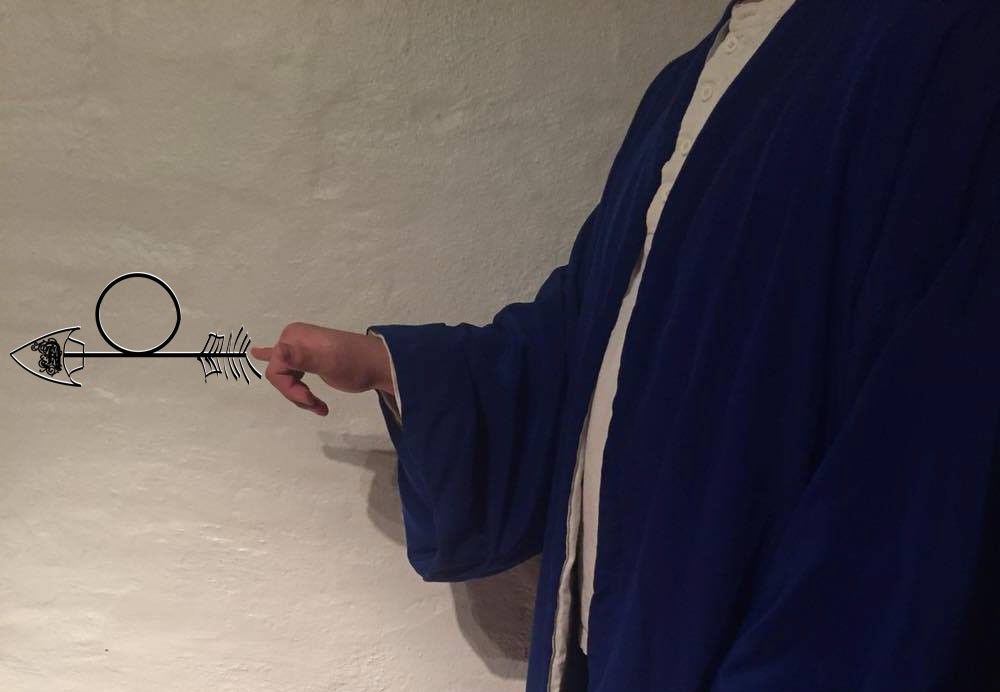
\includegraphics[width=\textwidth]{mainstuff/riteBilleder/Tanke.png}
\Large \textbf{Navn:} Tanke\\
\textbf{Rite:} Mentalis\\
\textbf{Bevægelse:} Tommelfinger og lillefinger strækkes ud mens resten knyttes. Hånden føres i en jævn bevægelse ind imod kroppen og derefter væk fra kroppen.
\end{rite*}

\begin{rite*}[Trække]
    \centering
    \includegraphics[width=\textwidth]{mainstuff/riteBilleder/Trække.png}
\Large \textbf{Navn:} Trække\\
\textbf{Rite:} Tran\\
\textbf{Bevægelse:} Hånden formes som en skål og føres fra brystet mod navlen.
\end{rite*}

\begin{rite*}[Vand]
    \centering
    
\includegraphics[width=\textwidth]{mainstuff/riteBilleder/Vand.png}
\Large \textbf{Navn:} Vand\\
\textbf{Rite:} Aqua\\
\textbf{Bevægelse:} Hånden formes således at den ser ud til at holde om en usynlig bold. Denne stilling føres nu først til højre og derefter til venstre
\end{rite*}
\end{document}